\documentclass[DM,lsstdraft,authoryear,toc]{lsstdoc}
\input{meta}

% Package imports
\usepackage{amsmath}
\usepackage{amssymb}
\usepackage{graphicx}
\usepackage{xspace}

% Local commands
\newcommand{\mur}{\ensuremath{\mu_r}\xspace}
\newcommand{\Reff}{\ensuremath{R_{\rm eff}}\xspace}
\newcommand{\Mstar}{\ensuremath{M_*}\xspace}
\newcommand{\Msun}{\ensuremath{M_\odot}\xspace}
\newcommand{\scarlet}{\textsc{scarlet}\xspace}
\newcommand{\scarletlite}{\textsc{scarlet-lite}\xspace}
\newcommand{\task}[1]{\texttt{#1}\xspace}

%If you want glossaries
%\input{aglossary.tex}
%\makeglossaries

\title{Quantifying the Performance of the LSST Detection and Deblending Pipeline: Implications for LSB Science and Beyond}

% This can write metadata into the PDF.
% Update keywords and author information as necessary.
\hypersetup{
    pdftitle={Quantifying the Performance of the LSST Detection and Deblending Pipeline: Implications for LSB Science and Beyond},
    pdfauthor={Thomas M. Sedgwick},
    pdfkeywords={LSST, deblending, source detection, low surface brightness, galaxy photometry, scarlet}
}

% Optional subtitle
% \setDocSubtitle{A subtitle}

\input{authors}

\setDocRef{DMTN-335}
\setDocUpstreamLocation{\url{https://github.com/lsst-dm/dmtn-335}}

\date{\vcsDate}

% Optional: name of the document's curator
% \setDocCurator{The Curator of this Document}

\setDocAbstract{%
We assess the LSST detection and deblending pipeline using source injection
experiments on real LSSTCam imaging (data release
\texttt{w\_2025\_37/DM-52496}). Mock NewHorizon galaxies
\citep{Martin2022} are injected into calibrated single-exposure images,
processed through the full pipeline to produce deep coadds, and the
resulting catalogues compared against those from unmodified coadds. Injected
sources span $18 < \mur < 30$~$\mathrm{mag\,arcsec^{-2}}$,
$1 < \Reff < 40$~arcsec, and $10^7 < \Mstar/\Msun < 10^{11.5}$.
%
We find: (i)~detection completeness drops from ${\sim}95\%$ at $\mur = 20$
to ${\sim}50\%$ at $\mur = 25$ and ${\sim}10\%$ at $\mur = 27$;
(ii)~for realistic sources, recovered $r$-band flux is overestimated by
${\sim}100\%$ at $\mur = 27$ and by an order of magnitude at $\mur = 30$;
(iii)~at fixed $\Reff = 5$~arcsec, flux is increasingly underestimated at
fainter surface brightnesses; (iv)~2D $\mur$--\Reff analysis shows flux
underestimation is driven by extendedness, with $\Reff > 15$~arcsec sources
underestimated by $40$--$100\%$; (v)~injecting a bright source ($\mur = 18$)
causes ${\sim}60\%$ of nearest-neighbour detections to be lost; (vi)~these
biases distort the galaxy stellar mass function below
$\log(\Mstar/\Msun) \sim 9$; (vii)~a dedicated experiment injecting
ICL-like core-S\'{e}rsic profiles with $R_e$ up to 60~arcsec produces
${\sim}10^3$ spurious detections and a comparable loss of real sources in
the most extended and brightest cases, with the summed flux of new
detections exceeding the injected flux by more than an order of magnitude,
and with the median flux of sources embedded in the ICL overestimated by a factor 10-100\%.  
%
These biases have ramifications for LSB science, weak lensing shear calibration,
environmental studies, photometric redshifts, transient host-galaxy association and more. We outline
next steps for mitigation within the Science Pipelines.
}

% Change history defined here.
% Order: oldest first.
% Fields: VERSION, DATE, DESCRIPTION, OWNER NAME.
% See LPM-51 for version number policy.
\setDocChangeRecord{%
  \addtohist{1}{YYYY-MM-DD}{Unreleased.}{Sedgwick}
}


\begin{document}

% Create the title page.
\maketitle
% Frequently for a technote we do not want a title page  uncomment this to remove the title page and changelog.
% use \mkshorttitle to remove the extra pages

% =============================================================================
\section{Introduction}
\label{sec:introduction}
% =============================================================================

The Vera C. Rubin Observatory Legacy Survey of Space and Time \citep[][]{Ivezic2019}
will image approximately 18\,000~deg$^2$ of
the southern sky in six broadband filters ($ugrizy$) over a ten-year survey,
reaching a co-added $5\sigma$ point-source depth of $r \sim 27.5$~mag. The
resulting photometric catalogues will underpin a broad range of science, from
precision cosmology through weak gravitational lensing
\citep[e.g.][]{LSST_DESC2018,Mandelbaum2018}, to galaxy evolution through
measurements of the galaxy stellar mass function
\citep[GSMF; e.g.][]{Baldry2012,Kelvin2014}, to time-domain science through
the association of transients with their host galaxies
\citep[e.g.][]{Foley2013}. The accuracy of these catalogues depends
critically on the fidelity of the source detection and deblending stages of
the data reduction pipeline.

Source detection is the first step
in constructing source catalogues from Rubin imaging. Any source that is not detected is entirely absent
from downstream science analyses, introducing hard selection effects that are
difficult to characterise after the fact. Detection algorithms must balance
sensitivity against contamination: thresholds that are too conservative will
miss faint or extended sources such as ultra-diffuse galaxies
\citep[UDGs;][]{vanDokkum2015}, classical low surface brightness (LSB)
galaxies \citep[e.g.][]{ImpeyBothun1997}, and dwarf galaxies
\citep[e.g.][]{Benson2003,Martin2019}, while thresholds that are too
aggressive produce spurious detections that contaminate catalogues,
cause extended sources such as intracluster
light (ICL); the diffuse stellar component of galaxy clusters
\citep[e.g.][]{Montes2019}; and well-resolved galaxies to be shredded into multiple sources.

The surface brightness depth of Rubin deep coadds, even at these early stages of the project,
exacerbates this tension: the population of LSB galaxies is predicted to
vastly outnumber the high surface brightness galaxy population, yet these are
precisely the objects most vulnerable to being missed. Their absence from
catalogues would directly bias the faint-end slope of the luminosity and
stellar mass functions, which in turn constrain models of galaxy formation,
feedback processes, and the nature of dark matter
\citep[e.g.][]{BullockBoylanKolchin2017}.

This surface brightness is also such
that the majority of detected objects lie in blends with at least one
neighbouring source. Deblending, the process of disentangling the flux
contributions of overlapping sources, is therefore not a corner-case
correction but a fundamental step in catalogue construction. Errors in
flux attribution propagate directly into photometric measurements, and from there
into derived quantities including photometric redshifts
\citep[e.g.][]{Benitez2000}, stellar masses
\citep[e.g.][]{Taylor2011,Bryant2015}, star formation rates, and shape
measurements used for weak lensing shear estimation
\citep[e.g.][]{SheldonHuff2017}. For strong lensing analyses, inaccurate
deblending of arcs and multiply-imaged sources can compromise lens modelling
and time-delay cosmography \citep[e.g.][]{Suyu2017}. In transient science,
mis-association of a supernova or other transient with the wrong host galaxy
due to deblending errors propagates into incorrect host-galaxy properties and
potentially biased cosmological inferences \citep[e.g.][]{Gupta2016,Sako2018}.
In addition, it is intuitive to expect any such biases to correlate with environment,
as blend complexity increases in dense environments. 
Similarly, measurements of ICL require the deblender to correctly apportion flux
between cluster member galaxies and the diffuse ICL component; failures in
this apportionment directly bias ICL fraction estimates and the inferred
assembly histories of clusters.

Detection and deblending are tightly coupled in the LSST Science Pipelines and
cannot be assessed in isolation. The detection stage determines the
\emph{footprints}; contiguous regions of pixels above threshold; and the
\emph{peaks} within them that seed the deblender. The quality of
the deblender's output therefore depends directly on the fidelity of the
detection stage: missed peaks leave flux unmodelled and either attributed to
neighbouring sources, or flux entirely attributed to the sky background, while spurious peaks cause the deblender to naively fragment
real objects or fit models to sky noise.

In this tech note, we present a systematic, quantitative assessment of the
performance of the current LSST detection and deblending pipeline. We use
controlled source injection experiments on real LSSTCam deep coadded imaging
to measure detection completeness and photometric bias in both injected sources and their real neighbours, 
as a function of surface brightness, effective radius, stellar mass, and local environment.
The structure of this note is as follows. In Section~\ref{sec:pipelines} we
describe the LSST Science Pipelines processing chain from single exposures to
detection, and explain how our injections enter at the
single-exposure level. In Section~\ref{sec:scarlet} we describe the
\scarletlite deblender, its role in the pipeline, and give a technical
overview of the algorithm. In Section~\ref{sec:failures} we
describe qualitative failure modes identified in real data that lead to our methodology. In
Section~\ref{sec:methodology} we detail our injection experiment methodology.
In Section~\ref{sec:results} we present our quantitative results. In
Section~\ref{sec:implications} we discuss implications for specific science
cases. In Section~\ref{sec:summary} we summarise our findings, and in
Section~\ref{sec:nextsteps} we outline next steps to help mitigate against the issues found.


% =============================================================================
\section{The LSST Science Pipelines: From Single Exposures to Catalogues}
\label{sec:pipelines}
% =============================================================================

The Rubin Science Pipelines \citep{Bosch2018,Bosch2019} process raw
single-exposure images through instrument signature removal (ISR), astrometric
and photometric calibration, and background subtraction, before combining
them into deep coadded images. In our injection experiments
(Section~\ref{sec:methodology}), we inject synthetic sources into calibrated (post-ISR)
single-exposure images prior to coaddition. These modified exposures are then
processed through the full pipeline exactly as any other LSST image would be,
producing deep coadds that contain our injected sources. We run source
detection and deblending on these modified coadds and compare the resulting
catalogues against those derived from the original, unmodified coadds. We
outline below the pipeline stages relevant to this workflow.

\subsection{Coaddition}
\label{sec:coaddition}

Calibrated single-epoch exposures are resampled onto the common pixel grid of
a pre-defined skymap (in our case, \texttt{lsst\_cells\_v1}) via the
\task{makeWarp} task, producing per-visit warped images
(\texttt{deepCoadd\_directWarp}). These warps are then combined into deep
coadds by the \task{assembleCoadd} task, which computes a weighted mean with
optional outlier rejection. Each coadd patch covers a sub-region of a tract
and is produced independently per band. The single exposures used in this work
are drawn from LSSTCam data release \texttt{w\_2025\_37/DM-52496}, processed
with the associated pipeline version.

\subsection{Detection}
\label{sec:detection}

Source detection on each per-band coadd is performed by
\task{DetectCoaddSourcesTask}, which first scales the variance plane to
account for noise correlations introduced during warping, then runs
\task{SourceDetectionTask} to identify contiguous regions of pixels above a
configurable signal-to-noise threshold. Each such region constitutes a
\emph{Footprint}, within which \emph{Peaks} are identified. The per-band
detection catalogues are then merged across all bands by
\task{MergeDetectionsTask}, which produces a single cross-band master source
list (\texttt{deepCoadd\_mergeDet}) with consistent source identifiers.
During this merge, spurious peaks around bright sources are culled according
to the \texttt{CullPeaksConfig} criteria. It is this merged catalogue of
Footprints and Peaks that is passed to the deblender.

% =============================================================================
\subsection{Deblending with Scarlet-lite}
\label{sec:scarlet}
\label{sec:deblending_meas}
% =============================================================================

The merged detection catalogue is passed to the \task{ScarletDeblendTask}
(from the \texttt{lsst.meas.extensions.scarlet} package), which performs
multiband deblending using the \scarletlite algorithm.
\scarletlite is a streamlined reimplementation
of the \scarlet deblending framework \citep{Melchior2018}, designed to operate
within the memory and runtime constraints of the LSST production pipeline. The
underlying models and optimisation algorithms are identical to those in
\scarlet; the differences are purely architectural, with \scarletlite assuming
that all bands share a common pixel grid and WCS, enabling analytic gradient
computation without an external automatic differentiation package.

Each footprint arriving from the detection stage is treated as an independent blend
scene: the deblender fits a multiband model to every peak 'source' within the Footprint
simultaneously, apportioning flux among the constituent sources. Each source is fitted with either one colour (single `SED') or two colours.
Often these 2 components take the form of a bulge and disc component of distinct colour, however no bulge-disc prior is implemented,
and these components can take any morphological form relative to each other,
with the only constraint being that they must be monotonically decreasing in flux from the centroid position found by detection.
The deblended source models are then used as templates for photometric measurement by
\task{MeasureMergedCoaddSourcesTask}, which measures fluxes, morphologies, and other
source properties in each band. Finally, \task{MergeMeasurementsTask} combines
the per-band measurements into the multi-band object catalogue
(\texttt{objectTable}). Sections~\ref{sec:matrix_factorisation} through \ref{sec:agnostic} give a more in depth overview of the algorithms utilised by \scarletlite.

\subsubsection{Constrained Matrix Factorisation}
\label{sec:matrix_factorisation}

\scarlet models the observed multi-band scene as a sum of $K$ source
components, each factorised into a spectral component (SED) $\mathbf{A}_k$
and a spatial morphology $\mathbf{S}_k$. The model $\mathbf{M}$ is expressed
as:
\begin{equation}
  \mathbf{M} = \mathbf{A}\mathbf{S} = \sum_{k=1}^{K} \mathbf{A}_k \otimes \mathbf{S}_k ,
  \label{eq:scarlet_model}
\end{equation}
where $\mathbf{A}_k$ is the SED vector of length equal to the number of
bands, specifying the flux in each filter for component $k$, and
$\mathbf{S}_k$ is a 2D image describing the spatial flux distribution of
component $k$. The outer product of the SED vector $\mathbf{A}_k$ and the
morphology image $\mathbf{S}_k$ yields a multi-band model cube for each
component; the full model $\mathbf{M}$ is the sum over all $K$ components,
or equivalently the matrix product $\mathbf{AS}$. When comparing the model
to the observed data, each component is convolved with the band-dependent
PSF\@. \scarlet solves for $\mathbf{A}_k$ and $\mathbf{S}_k$ simultaneously
across all bands by minimising a $\chi^2$ loss function under a set of
physically motivated constraints \citep{Melchior2018}.

\subsubsection{Optimisation: Proximal Gradient Descent}
\label{sec:optimisation}

The minimisation is performed using the adaptive proximal gradient method
(AdaProx; a non-smooth generalisation of the ADAM optimiser), implemented in
the \texttt{proxmin} library \citep{MoolekampMelchior2018}. In each
iteration, the algorithm: (1)~computes the gradient of the $\chi^2$ loss
with respect to both $\mathbf{A}_k$ and $\mathbf{S}_k$; (2)~takes a downhill
step with an adaptive step size; and (3)~applies proximal operators to
enforce each constraint. This forward-backward splitting approach (also known
as ISTA/FISTA in the convex case) allows the incorporation of
non-differentiable constraints through their proximal operators, which project
the current iterate onto the feasible set defined by the constraint
\citep{ParikhBoyd2014}.

\subsubsection{Constraints}
\label{sec:constraints}

\textbf{Non-negativity.}\ Both $\mathbf{A}_k$ and $\mathbf{S}_k$ are
constrained to be non-negative, reflecting the physical requirement that
source fluxes cannot be negative.

\textbf{Monotonicity.}\ The morphology $\mathbf{S}_k$ is constrained to be
monotonically decreasing from the peak pixel. This is implemented via a
proximal operator that enforces, for each pixel, that its value does not
exceed the weighted mean of its neighbours lying closer to the peak
\citep{Melchior2018}. Three weighting schemes are available, with the default
(`angle' weighting) combining three neighbour pixels closer to the peak to
reduce radial spike artefacts. While this constraint is physically
well-motivated for smooth elliptical galaxies, it is a poor approximation for
sources with star-forming regions, spiral arms, or other non-monotonic
features. Crucially, this means that a single \scarlet component cannot
represent a galaxy with localised bright regions away from the nucleus.

\textbf{Symmetry (optional).}\ An optional 180-degree rotational symmetry
constraint can be applied to the morphology, enforcing $S_k(x,y) =
S_k(-x,-y)$ relative to the peak. The proximal operator for this constraint
replaces each symmetric pixel pair with their mean. In the default LSST
pipeline configuration, symmetry is not enforced.

\textbf{Component structure.}\ \scarlet permits up to two
\texttt{FactorisedComponent} instances per source (e.g.\ representing a bulge
and a disk), each with an independent SED and morphology. These are combined
via \texttt{CombinedComponent}. More complex galaxies with strong colour
gradients or multiple stellar populations are therefore represented by at most
two spectral-morphological components, which limits the fidelity of the model
for sources with, e.g., three or more distinct colour regions.

\subsubsection{Initialisation and Convergence}
\label{sec:initialisation}

Source morphologies are initialised from the detection Footprint and the
observed pixel data. The SED is initialised by extracting the multi-band flux
at the Peak position. \scarlet then iterates the proximal gradient descent
until the fractional change in the loss function falls below a configurable
convergence threshold (controlled by the \texttt{ScarletDeblendConfig}
parameters, including \texttt{maxIter} and \texttt{relativeError}). If a
source fails to initialise (e.g.\ due to insufficient signal), \scarlet can
optionally fall back to a model with fewer components.

\subsubsection{PSF Handling and Photometry}
\label{sec:psf_handling}

\scarlet operates on PSF-convolved models: each component model
$\mathbf{A}_k \cdot \mathbf{S}_k$ is convolved with the band-dependent PSF
$\mathbf{P}_b$ before comparison with the data. This allows \scarlet to
handle variable seeing across bands naturally. The deconvolved model (i.e.\
the intrinsic source model before PSF convolution) is stored as a
\texttt{ScarletModelData} object in the Butler datastore, enabling post-hoc
reprocessing without re-running the optimisation. The model yields consistent
multiband deblended fluxes in each band, with the multiband fit providing
cross-band regularisation.

\subsubsection{Key Limitation: Agnosticism to Detection Legitimacy}
\label{sec:agnostic}

A critical feature of \scarlet is that it is entirely agnostic to the
legitimacy of the input Peaks. Every Peak in the merged detection catalogue
is treated as a real source and is assigned a share of the observed flux. If
the detection pipeline places spurious Peaks within a single galaxy (e.g.\ on
spiral arms, tidal features, or noise fluctuations), \scarlet will model each
of these as an independent source. This design means that any shortcomings in
the upstream detection and peak-finding stages propagate directly into
deblending artefacts, most notably the shredding of extended sources.


% =============================================================================
\section{Qualitative Failure Modes in Real Data}
\label{sec:failures}
% =============================================================================

Prior to designing our injection experiments, we examined the blending
environment in the LSST deep coadds and identified two principal failure modes
through visual inspection. Figure~\ref{fig:blend_complexity} shows the
distribution of blend complexity (number of Peaks per Footprint) in the deep
coadd catalogue: while the majority of Footprints contain a single Peak, a
substantial fraction contain two or more, and blends with five or more members
are not uncommon. The prevalence of blending underscores the importance of
robust deblending for LSST catalogue science.

\begin{figure}
  \centering
  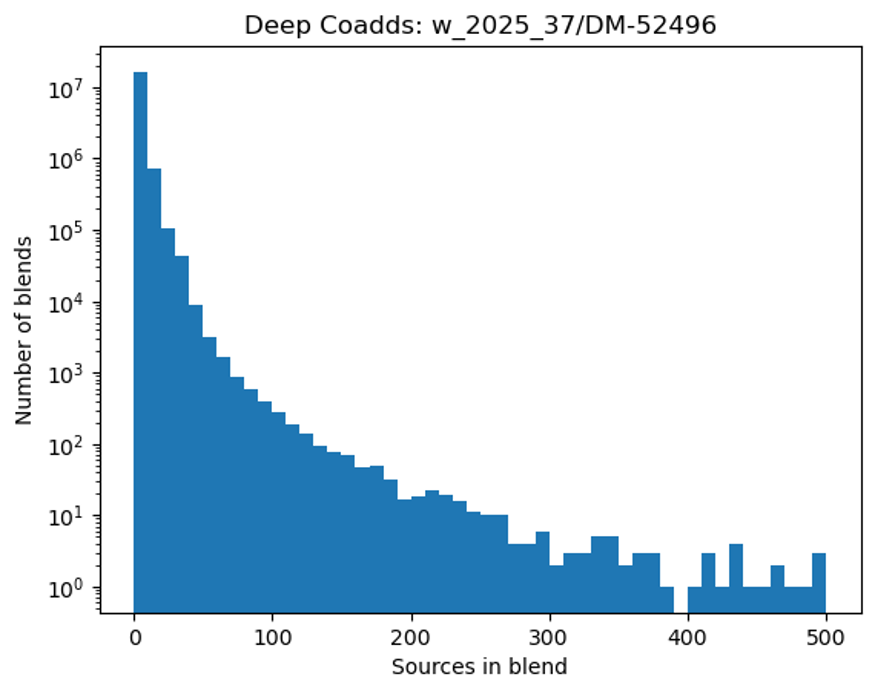
\includegraphics[width=0.85\textwidth]{figures/blend_complexity_distribution}
  \caption{Distribution of blend complexity (number of Peaks per Footprint)
    in the LSST deep coadd catalogue. The majority of Footprints contain a
    single Peak, but multi-peak blends are common, with a long tail extending
    to high multiplicity.}
  \label{fig:blend_complexity}
\end{figure}

\subsection{Left-behind Flux in Non-monotonic Sources}
\label{sec:leftbehind}

Figure~\ref{fig:left_behind} shows a representative blend containing an
extended late-type galaxy (source~19) with visible spiral structure. The
\scarlet model (middle panel) fails to capture the full extent of this source:
the residual (right panel) shows significant unmodelled flux in the spiral
arms and the bulge-disk transition region. This is a direct consequence of the
monotonicity constraint (Section~\ref{sec:constraints}), which prevents the
morphology model from representing localised flux enhancements (e.g.\
star-forming H\textsc{ii} regions, spiral arm segments) that lie above the
monotonically decreasing profile. Because \scarlet fits at most two SED
components, colour gradients across the disk-to-bulge transition are also
poorly captured, further contributing to the residual. The left-behind flux
will cause the integrated photometry of such sources to be systematically
underestimated.

\begin{figure}
  \centering
  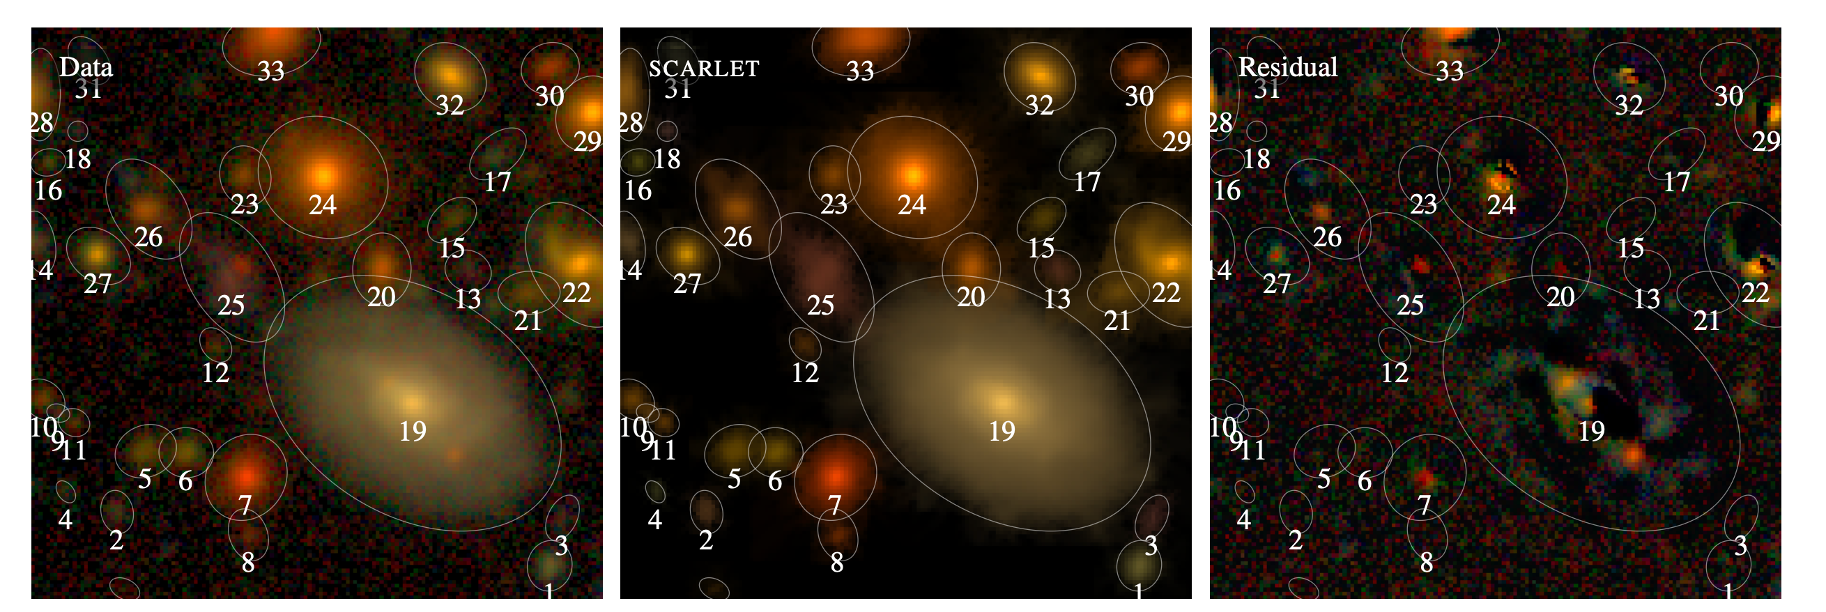
\includegraphics[width=\textwidth]{figures/leftbehind_flux_failure}
  \caption{Taken from \citet{Melchior2018}. Failure Mode~1: left-behind flux
    in a non-monotonic, multi-SED source. \textit{Left}: $gri$ colour composite
    of the observed blend with labelled source identifiers. \textit{Centre}:
    \scarletlite model. \textit{Right}: residual (data minus model). The
    residual around source~19 reveals unmodelled spiral arm flux and a
    bulge-disk colour gradient artefact, arising from the monotonicity
    constraint and the two-component SED limit.}
  \label{fig:left_behind}
\end{figure}

\subsection{Shredding of Extended Sources by Spurious Detections}
\label{sec:shredding}

Figure~\ref{fig:shredding} shows three examples of extended sources that have
been shredded by the deblender. In each case, the upstream
\task{DetectCoaddSourcesTask} has placed multiple Peaks within the Footprint
of a single galaxy. Because \scarlet is agnostic to detection legitimacy
(Section~\ref{sec:agnostic}), it assigns each Peak a model and a share of the
observed flux, splitting what should be a single source into several catalogue
entries. This failure mode is particularly severe for galaxies with tidal
streams, ICL envelopes, or asymmetric morphologies. The consequence is
twofold: the shredded parent galaxy has its flux underestimated, and the
catalogue is contaminated with spurious sources.

\begin{figure}
  \centering
  \includegraphics[width=\textwidth]{figures/shredding_extended_sources}
  \caption{Failure Mode~2: shredding of extended sources. $gri$ composite
    images of three blended scenes from real LSST deep coadds in which tidal
    streams, ICL, or asymmetric galaxy components have been misidentified as
    separate Peaks by the detection pipeline, causing the deblender to
    redistribute the host galaxy flux among spurious child sources. White
    numbers indicate a source considered to be in a blend with source~0. Red
    circles denote nearby detections not considered to be in the blend.}
  \label{fig:shredding}
\end{figure}


% =============================================================================
\section{Injection Experiment Methodology}
\label{sec:methodology}
% =============================================================================

To quantify the severity of the failure modes identified above,
we designed a suite of controlled injection experiments.
We inject synthetic galaxy images with known ground-truth photometric properties
into calibrated single-exposure images prior to coaddition,
so that the injected sources undergo identical processing to real sources,
including sky subtraction, co-addition weighting, PSF convolution, detection, deblending, and measurement.
We then compare the recovered catalogue properties against the input values and against the catalogues produced
from the unmodified coadds, isolating the pipeline's response to sources of known properties in a fully controlled manner.

\subsection{Synthetic Sources: NewHorizon Simulations}
\label{sec:newhorizon}

Our injected sources are drawn from the NewHorizon cosmological hydrodynamical
simulation \citep{Dubois2021,Martin2022}, which provides 37 spatially
well-resolved dwarf galaxies at $z = 0.05$ as six-band ($ugrizy$) image cubes.
These mock observations exhibit realistic morphological features including
non-monotonic flux profiles from star-forming regions, multi-component
disk-bulge structures, and asymmetric features. For the experiments presented
here, we restrict our injections to NewHorizon galaxies without resolved
satellite companions, in order to simplify the bookkeeping when tracking
detections before and after injection.

\begin{figure}
  \centering
  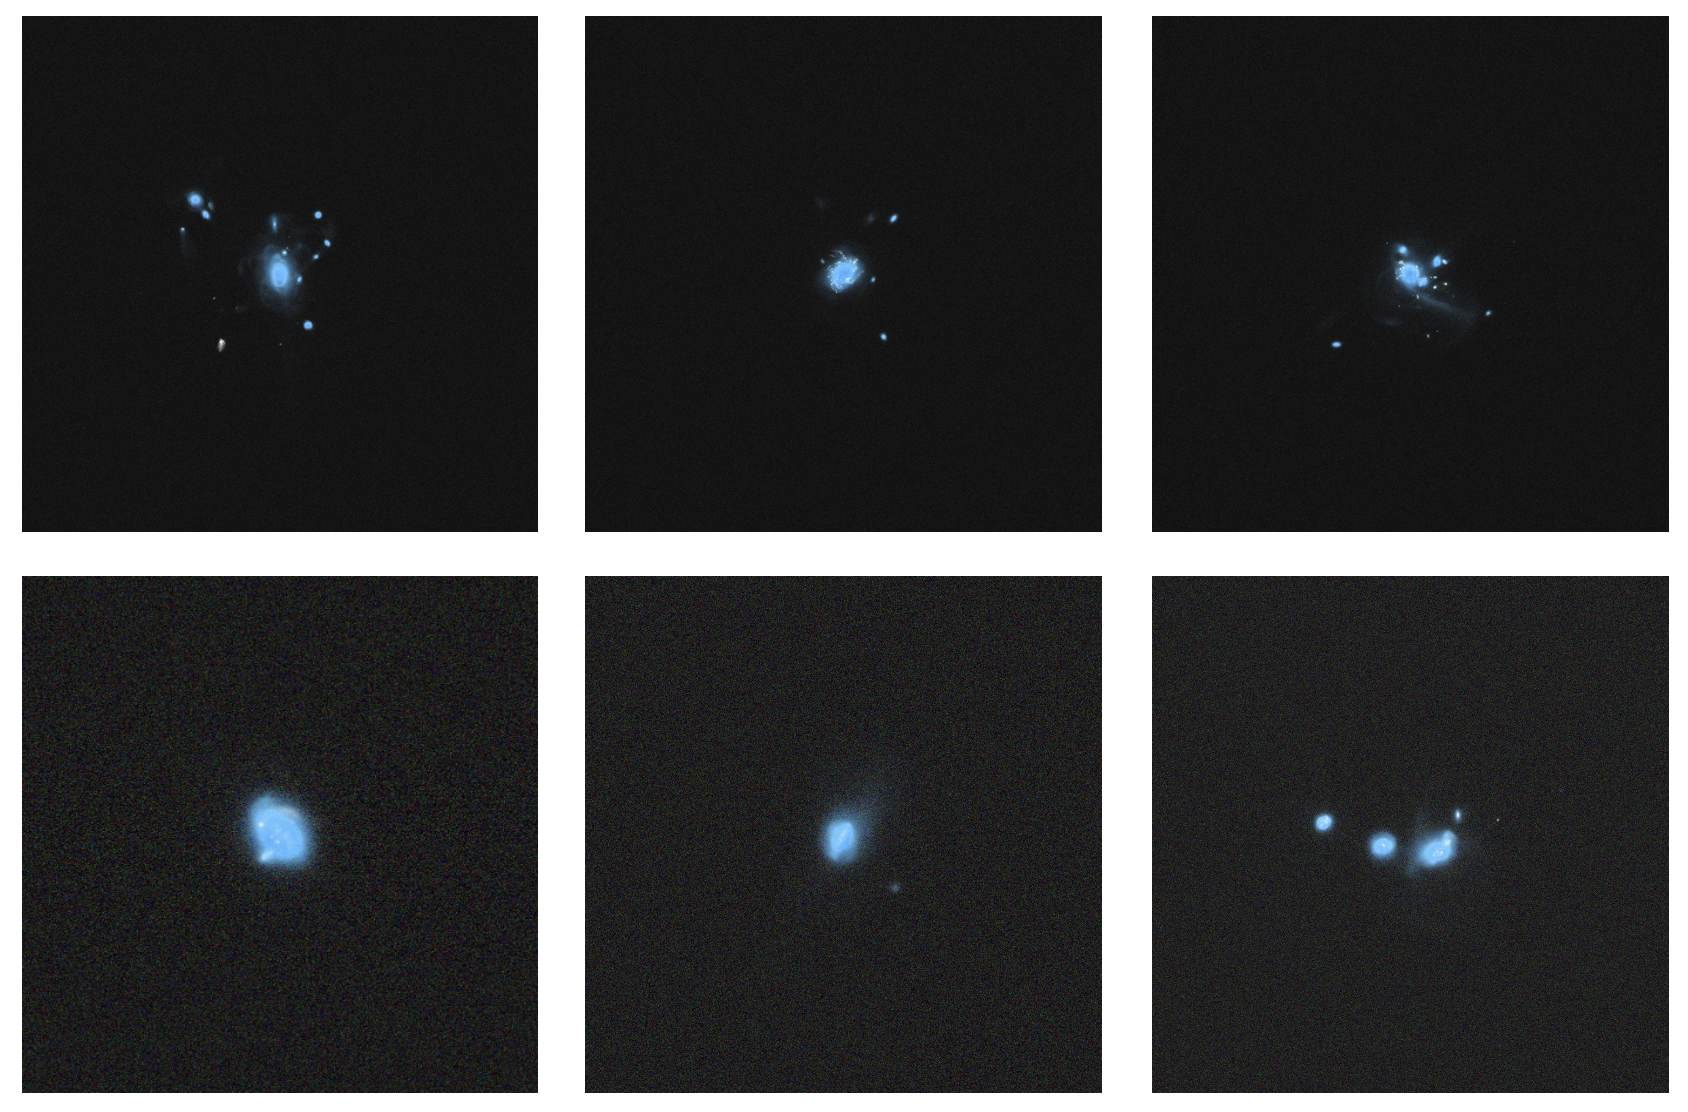
\includegraphics[width=0.9\textwidth]{figures/newhorizon_dwarf_galaxies}
  \caption{Mock observations ($gri$ composite image) of six NewHorizon
    simulated dwarf galaxies \citep{Martin2022} used as injection templates.}
  \label{fig:newhorizon}
\end{figure}

\subsection{Injected Galaxy Property Manipulation}
\label{sec:property_manipulation}

For each injection, we manipulate the NewHorizon image cube to achieve a
specified set of five target physical properties: $r$-band mean surface
brightness $\mur$ (defined as the mean surface brightness within \Reff),
effective radius \Reff, $u-r$ colour (a proxy for star formation rate),
photometric redshift $z$, and stellar mass $\log(\Mstar/\Msun)$.

The procedure is as follows. We first resize the image cube (via interpolation
and re-binning at the LSST pixel scale of 0.2~arcsec~px$^{-1}$) to achieve
the target PSF-convolved \Reff. The $r$-band flux is then scaled to achieve the
target $\mur$. The $u$-band flux is set from the target $u-r$ colour, and
the remaining band fluxes ($g, i, z, y$) are predicted from the target
photo-$z$ and $\log M_*$, where we use the \textsc{lephare} photo-$z$
prescription and the mass prescription of \citet{Bryant2015}:
\begin{equation}
  \log\!\left(\frac{M_*}{M_\odot}\right) = -0.4\,m_i + 0.4\,D + f(z) + g(z)\,(g-i)_{\rm obs} ,
  \label{eq:mass_prescription}
\end{equation}
where $D$ is the distance modulus, derived from the photo-$z$ using a flat
$\Lambda$CDM cosmology with $H_0 = 70$~km~s$^{-1}$~Mpc$^{-1}$,
$\Omega_\mathrm{m} = 0.3$, $\Omega_\Lambda = 0.7$, and $f(z)$, $g(z)$ are
polynomial functions of redshift. The injected image cube is convolved with
the per-band PSF for each single exposure.

\subsection{COSMOS-UltraVISTA Property Draws}
\label{sec:cosmos_draws}

For our primary experiment (Experiment~1), we seek to inject sources with
properties that are realistic for a given surface brightness bin. We use the
COSMOS-2020 UltraVISTA photometric catalogue \citep{Weaver2022} restricted to
$z < 0.4$ as our reference population. For each target $\mur$ (in bins of
0.5~$\mathrm{mag\,arcsec^{-2}}$ from 18 to 30), we select all COSMOS galaxies
within $\pm 0.25$~$\mathrm{mag\,arcsec^{-2}}$ of the target and fit a
multivariate kernel density estimate (KDE) to the joint distribution of eleven
quantities: the five source properties ($\log M_*$, $z$, $u-r$, $\log \Reff$,
$\mur$) of each COSMOS galaxy, the corresponding properties of their nearest
neighbour (NN), and the separation to these neighbours, in units of the
neighbour's effective radius. We draw 100 sets of galaxy properties from this
KDE, yielding 100 realistic injections per surface brightness bin.

\begin{figure}
  \centering
  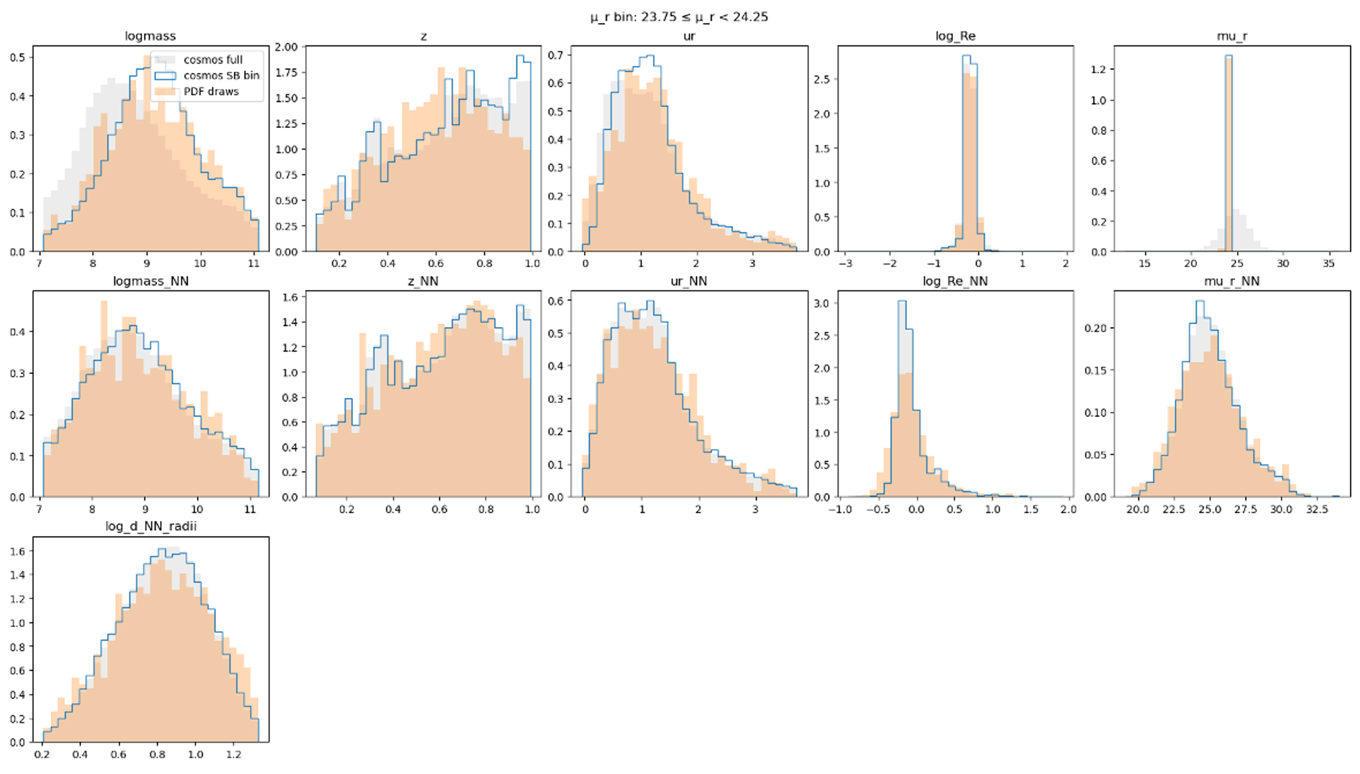
\includegraphics[width=\textwidth]{figures/cosmos_kde_marginals}
  \caption{Marginal distributions of injected source and nearest-neighbour
    properties drawn from the COSMOS-UltraVISTA KDE for the $\mur = 24$
    $\mathrm{mag\,arcsec^{-2}}$ bin. Grey: full COSMOS sample ($z < 0.4$).
    Blue outlines: COSMOS galaxies in the narrow $\mur$ bin. Orange filled:
    100 draws from the fitted KDE.}
  \label{fig:kde_marginals}
\end{figure}

\begin{figure}
  \centering
  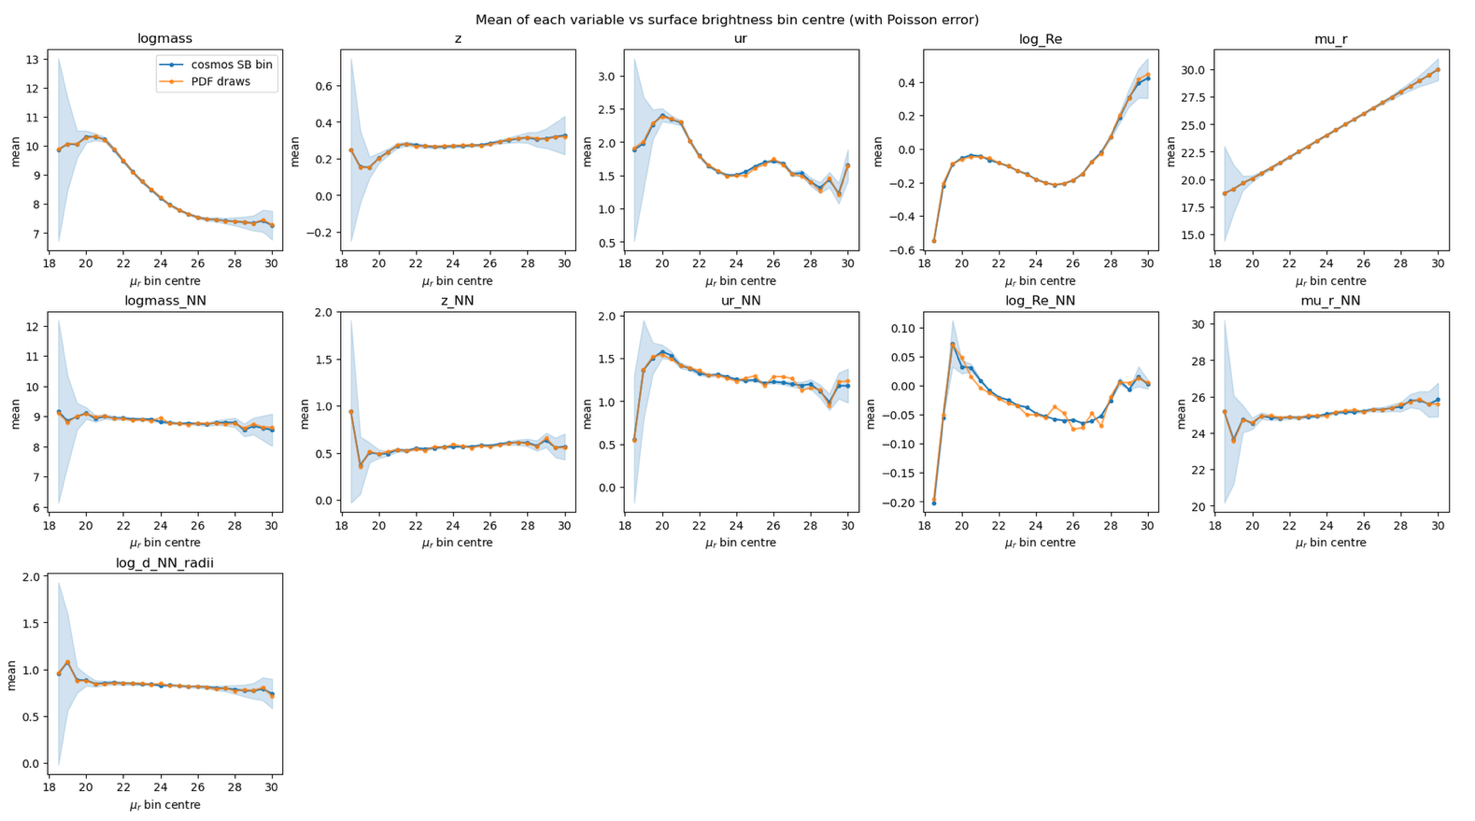
\includegraphics[width=\textwidth]{figures/cosmos_mean_properties_vs_sb}
  \caption{Mean properties of the reference COSMOS-UltraVISTA $z < 0.4$
    source sample as a function of $r$-band surface brightness (blue line).
    The list of properties is the same as shown in Figure~\ref{fig:kde_marginals}.
    The standard deviation on each property is shown as the blue filled region.
    The mean properties of the 100 random draws from the PDFs at each surface
    brightness bin are shown in orange.}
  \label{fig:cosmos_properties}
\end{figure}

\subsection{Injection Locations and Environment Matching}
\label{sec:injection_locations}

For each drawn set of galaxy properties, we identify a host location in the
real LSST coadd by querying the object catalogue (\texttt{objectTable}) for
the galaxy whose properties ($z$, $\log M_*$, $\mur$, $\log \Reff$) best
match the drawn nearest-neighbour properties. This matching is performed using
a $k$-d tree with hard similarity cuts on $z$ ($\pm 0.1$), $\log M_*$
($\pm 0.5$~dex), $\mur$ ($\pm 1$~$\mathrm{mag\,arcsec^{-2}}$), and
$\log \Reff$ ($\pm 0.5$~dex), and equal weighting given to each variable. The
injected source is then placed at the drawn separation $d_{\rm NN}$ (in arcsec)
from the matched host, at a random position angle. If no position angle would
result in this galaxy still being the nearest neighbour to our injected galaxy,
we skip this galaxy and proceed to the next best match to our target NN
properties, repeating until a successful injection is achieved.

\subsection{Pipeline Execution and Source Matching}
\label{sec:source_matching}

After the modified single exposures are processed through the pipeline to
produce coadds, we run \task{SourceDetectionTask} and
\task{ScarletDeblendTask} on the modified \texttt{MultibandExposure}. We
cross-match the output detection catalogue against the injection position
(within a tolerance of 5~pixels, i.e.\ 1~arcsec) to determine whether the
injected source was detected. For detected injections, we record the recovered
$r$-band \scarlet model flux (the \texttt{modelFlux} field from the deblended
source catalogue) and compute the fractional flux bias as
$(f_{\rm recovered} - f_{\rm injected}) / f_{\rm injected}$. We also track
whether the pre-injection nearest neighbour (the object used to decide where
to inject) survives detection in the post-injection catalogue (within a
5-pixel matching radius), and record its flux and stellar mass bias. We also
track the full rest-of-blend population (all other sources in the same parent
Footprint) to quantify the collateral impact on the photometry of real sources.

\subsection{Example Injections In Situ}
\label{sec:example_injections}

Figure~\ref{fig:injections_bright} shows a simplified example of injections
at $\mur = 20$~$\mathrm{mag\,arcsec^{-2}}$, at the same injection position
and using the same NewHorizon galaxy.
Figure~\ref{fig:injections_faint} shows the more detailed approach (for
$\mur = 24$~$\mathrm{mag\,arcsec^{-2}}$) of injecting at a range of
positions using the method described in Section~\ref{sec:injection_locations},
and using a random NewHorizon galaxy for each injection.

\begin{figure}
  \centering
  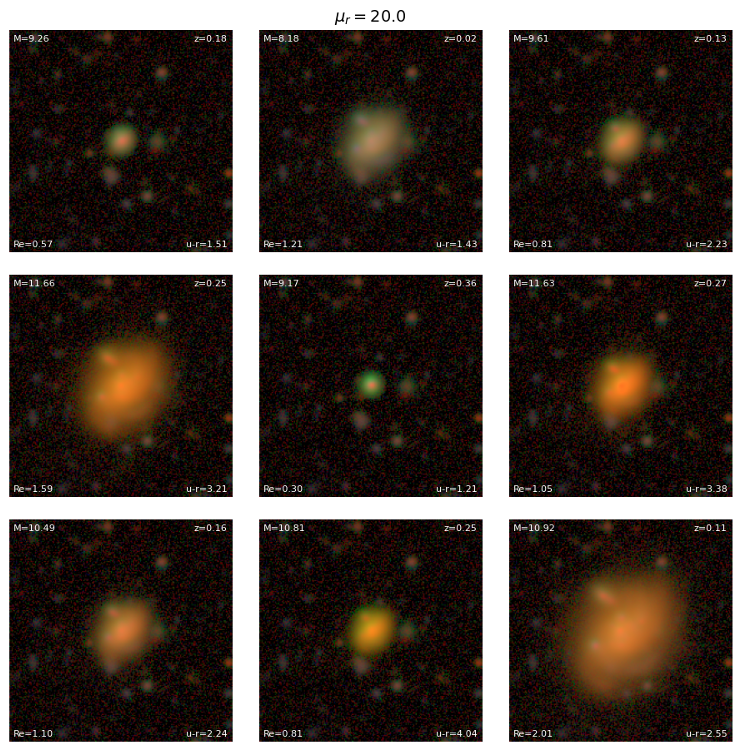
\includegraphics[width=\textwidth]{figures/injections_bright_sb20}
  \caption{Nine example injections at $\mur = 20.0$~$\mathrm{mag\,arcsec^{-2}}$
    in real LSST deep coadds. Each stamp shows the same injected NewHorizon
    galaxy (ID:\,NH00125) with its $ugrizy$ fluxes and spatial resolution
    adjusted to meet the target set of properties (see
    Section~\ref{sec:property_manipulation}).}
  \label{fig:injections_bright}
\end{figure}

\begin{figure}
  \centering
  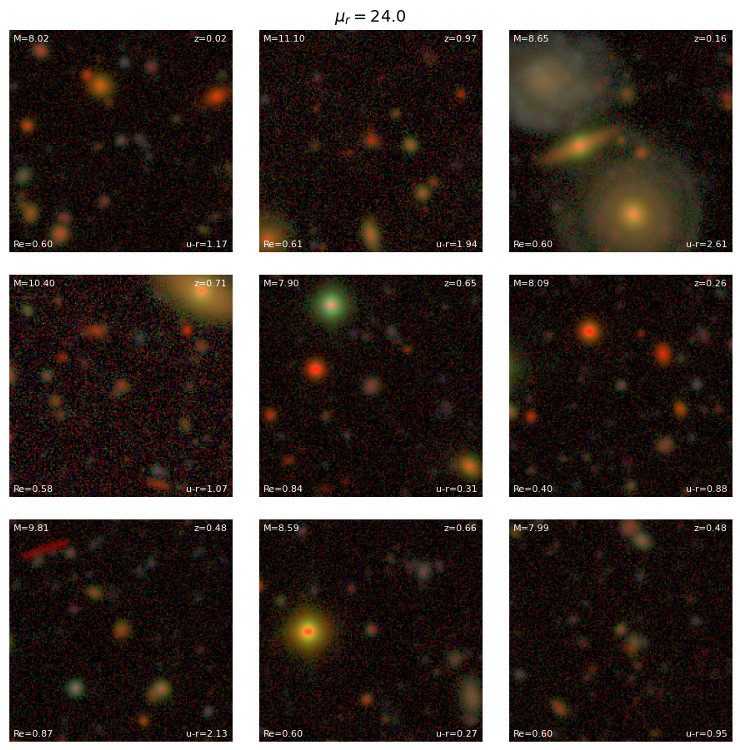
\includegraphics[width=\textwidth]{figures/injections_faint_sb24}
  \caption{As Figure~\ref{fig:injections_bright}, but for a target of
    $\mur = 24.0$~$\mathrm{mag\,arcsec^{-2}}$, and with injections at
    different locations and using different NewHorizon galaxies per injection.}
  \label{fig:injections_faint}
\end{figure}


% =============================================================================
\section{Results}
\label{sec:results}
% =============================================================================

\subsection{Qualitative Example: Before and After Injection}
\label{sec:before_after}

Figure~\ref{fig:before_after} shows a single blend before (left panels) and
after (right panels) injection of a bright NewHorizon galaxy at $\mur = 21$
$\mathrm{mag\,arcsec^{-2}}$ (iteration~3 of 100, highlighted with a red
circle). After injection, sources~9 through~13 have lost their detections
entirely: the bright injected source has expanded the parent Footprint and
the detection algorithm has failed to identify these fainter Peaks within the
merged blend. The \scarlet model for the injected source has extended well
beyond the true extent of the injection, consuming flux from the
now-undetected neighbours.

\begin{figure}
  \centering
  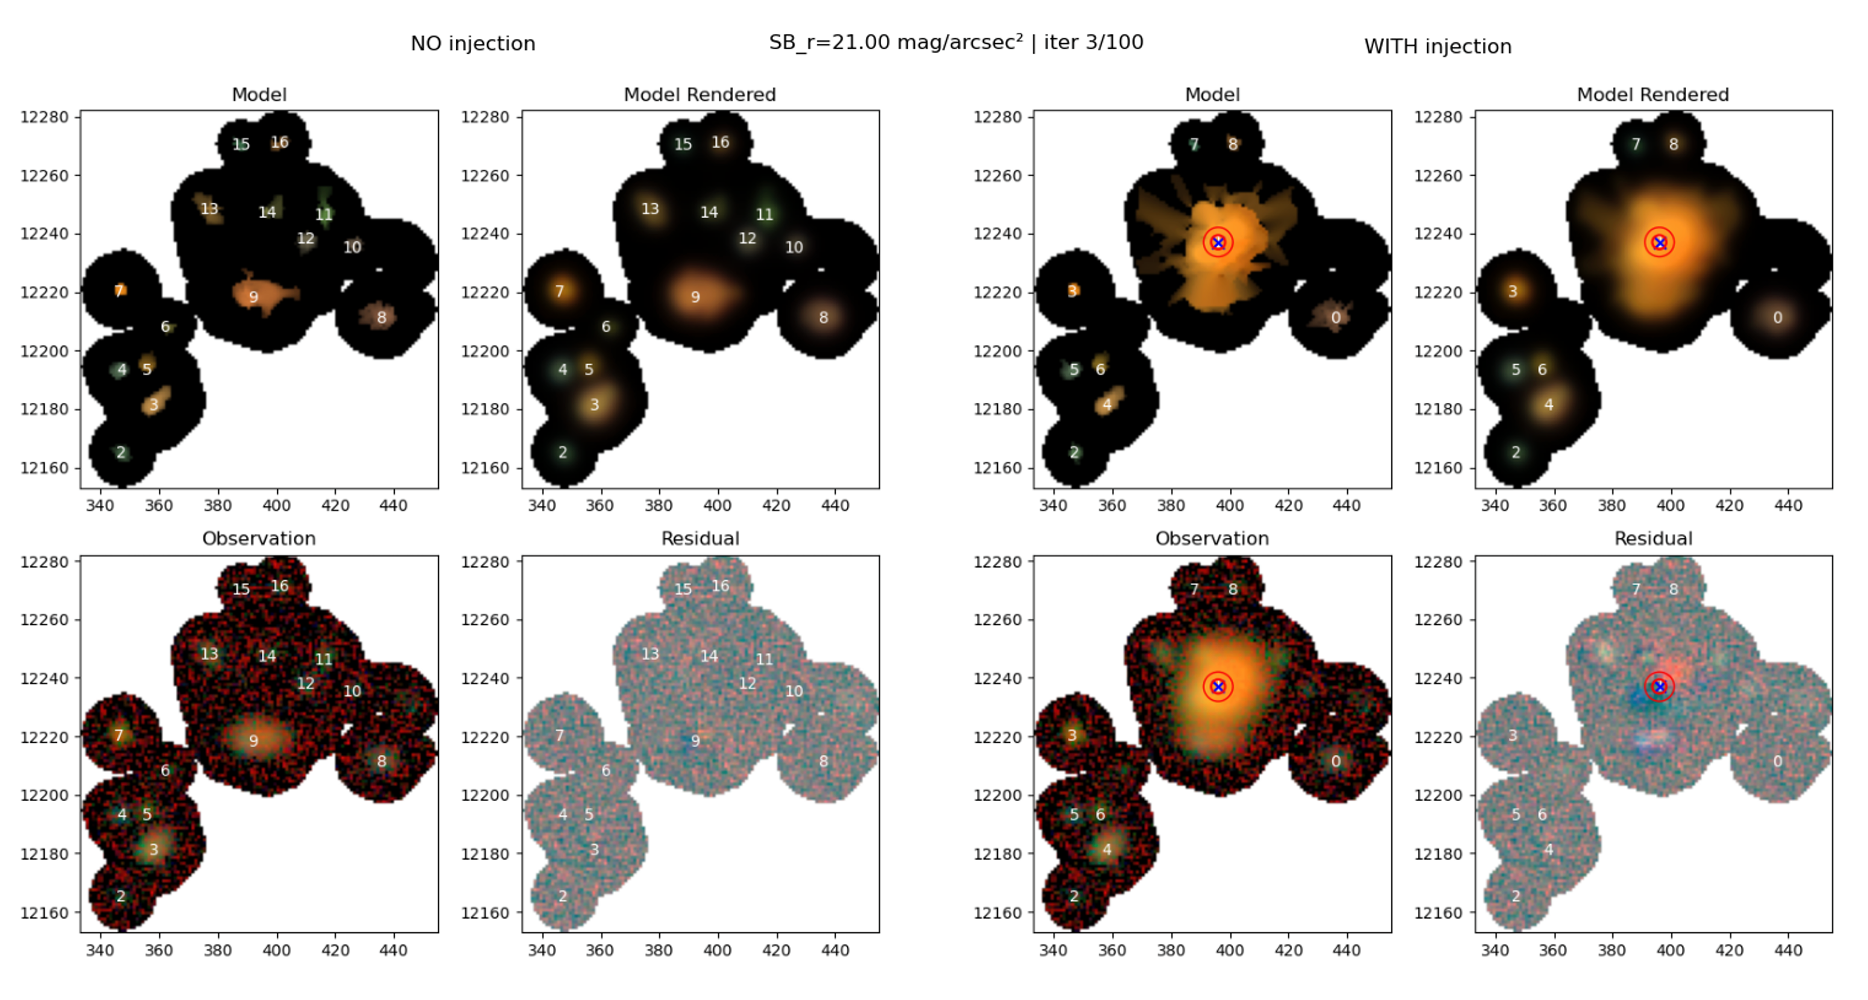
\includegraphics[width=\textwidth]{figures/blend_before_after_injection}
  \caption{A single blend before injection (left four panels: model, rendered
    model, observation, residual) and after the injection of a bright
    NewHorizon galaxy at $\mur = 21$~$\mathrm{mag\,arcsec^{-2}}$ (right four
    panels; injected source circled in red). Sources~9--13 have lost their
    detections due to the presence of the bright injected source.}
  \label{fig:before_after}
\end{figure}

\subsection{Experiment 1: Realistic Galaxies (COSMOS-drawn Properties)}
\label{sec:exp1}

Figure~\ref{fig:exp1_results} presents the aggregate detection and photometric
performance across all 100 injections per surface brightness bin, with galaxy
properties drawn from the COSMOS-UltraVISTA KDE
(Section~\ref{sec:cosmos_draws}).

\begin{figure}
  \centering
  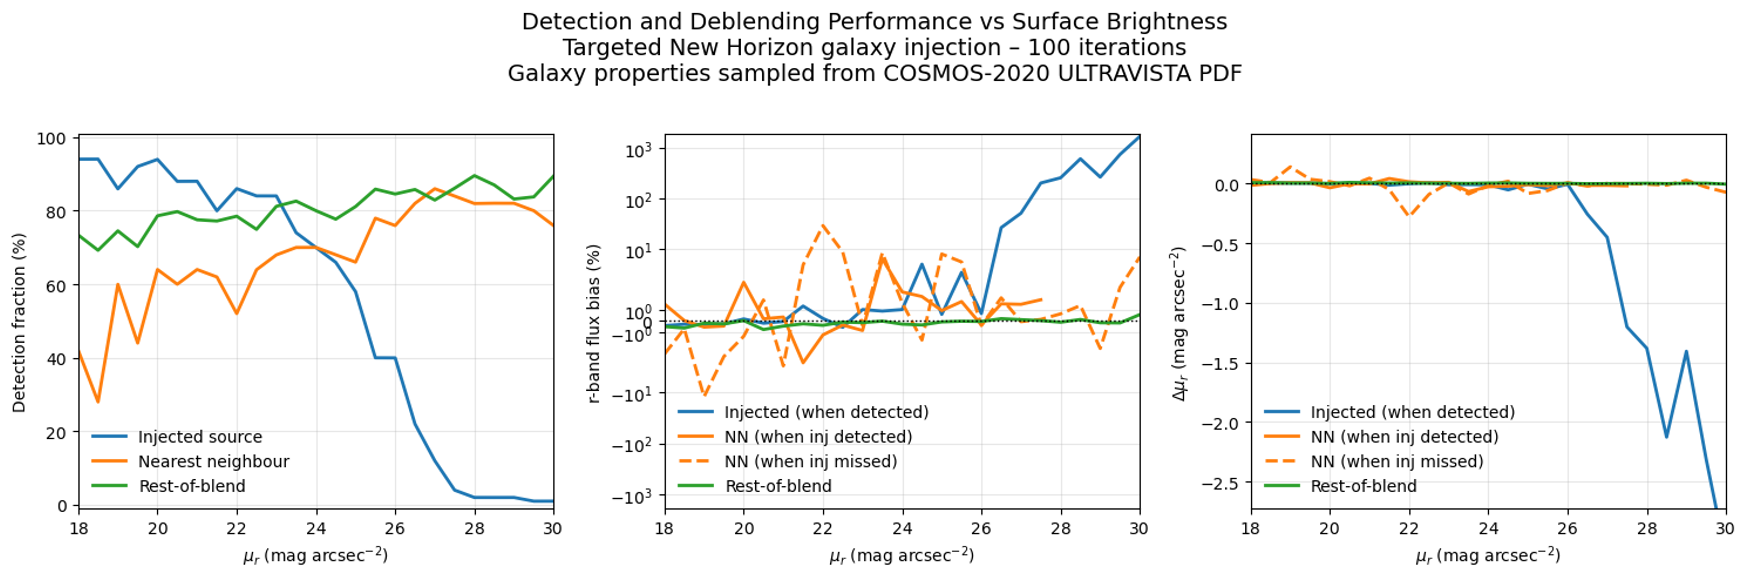
\includegraphics[width=\textwidth]{figures/exp1_detection_flux_bias}
  \caption{Detection and deblending performance vs.\ $r$-band surface
    brightness for Experiment~1 (COSMOS-drawn galaxy properties, 100
    injections per bin). \textit{Left}: detection fraction. \textit{Centre}:
    median $r$-band flux bias. \textit{Right}: median surface brightness
    bias in $\mathrm{mag\,arcsec^{-2}}$.}
  \label{fig:exp1_results}
\end{figure}

\subsubsection{Detection Completeness}
\label{sec:detection_completeness}

The injected-source detection fraction (blue, left panel) is $90$--$95\%$
for $\mur < 22$~$\mathrm{mag\,arcsec^{-2}}$, declining to approximately
$50\%$ at $\mur = 25$ and to ${\sim}10\%$ at $\mur = 27$. The $50\%$
completeness limit at $\mur \sim 25$ represents the effective surface
brightness limit of the current detection pipeline for resolved sources in
typical blending environments. The nearest-neighbour detection fraction
(orange) reveals a striking secondary effect: at the brightest injection
surface brightnesses ($\mur \sim 18$), approximately $60\%$ of nearest
neighbours are lost. This fraction recovers to ${\sim}80\%$ for faint
injections ($\mur > 26$), but never reaches $100\%$, indicating that even a
faint injection perturbs the detection of nearby sources at the ${\sim}20\%$
level.

\subsubsection{Photometric Bias}
\label{sec:photometric_bias}

The $r$-band fractional flux bias of the injected source (centre panel) is
consistent with zero for $\mur < 25$~$\mathrm{mag\,arcsec^{-2}}$. Beyond
this, the recovered flux increasingly overestimates the input: the bias
reaches ${\sim}{+}100\%$ (recovered flux approximately twice the input) at
$\mur \sim 27$, and approximately an order of magnitude at $\mur = 30$
(i.e.\ recovered flux is ${\sim}10$ times the input, corresponding to a bias
of $+900\%$). In magnitude space, a factor-of-10 flux overestimate
corresponds to ${\sim}2.5$~mag. The right-hand panel shows the corresponding
surface brightness bias: for the few sources detected at $\mur > 27$ (where
$N_{\rm det}$ is small), the recovered surface brightness is
$1.5$--$2.5$~$\mathrm{mag\,arcsec^{-2}}$ brighter than the input.

\subsection{Experiment 2: Surface Brightness in Isolation}
\label{sec:exp2}

Experiment~1 varies all galaxy properties simultaneously as a function of
surface brightness, following the correlated COSMOS distributions. To isolate
the effect of surface brightness alone, we repeat the experiment with all
other properties held fixed: $\Reff = 5$~arcsec, $u-r = 1.25$~mag, $z =
0.1$, $\log(\Mstar/\Msun) = 9.0$.

\begin{figure}
  \centering
  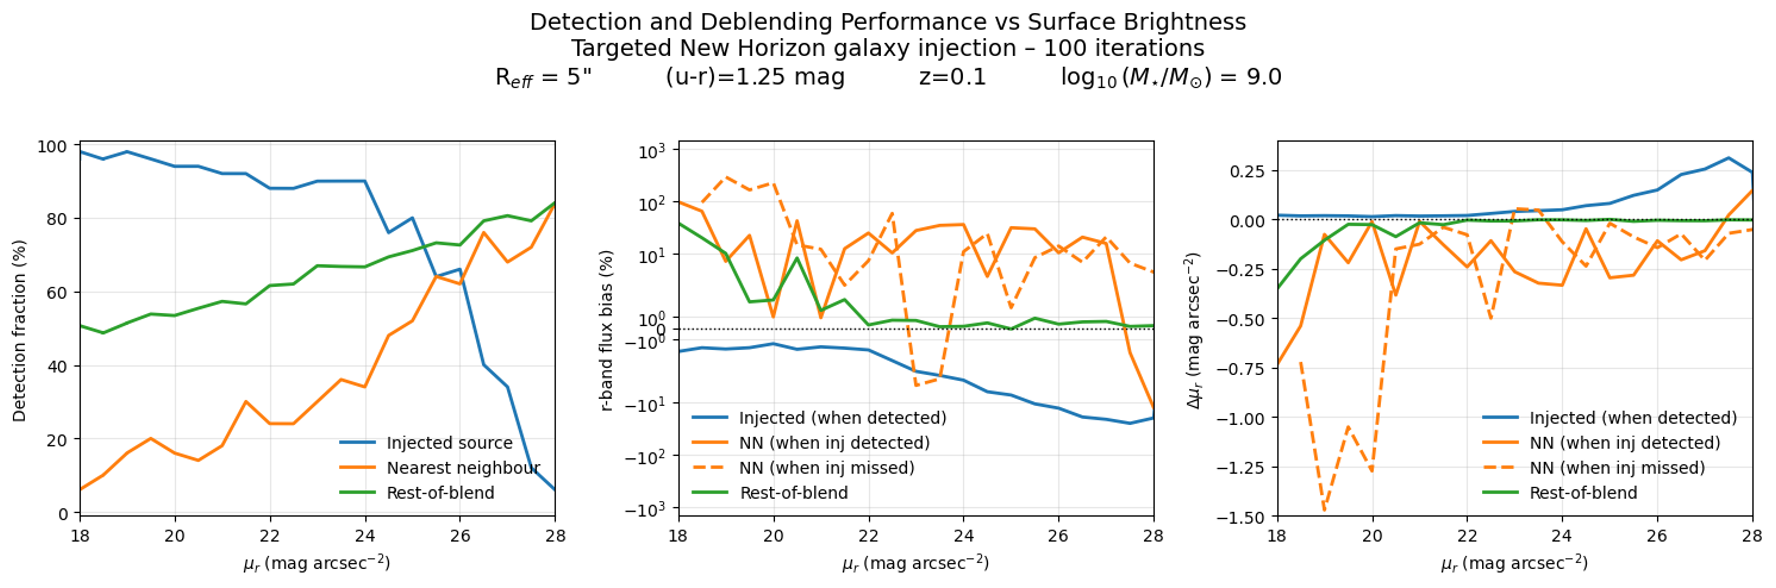
\includegraphics[width=\textwidth]{figures/exp2_detection_flux_bias}
  \caption{As Figure~\ref{fig:exp1_results}, but for Experiment~2: only
    surface brightness is varied; $\Reff = 5$~arcsec, $u-r = 1.25$~mag, $z
    = 0.1$, $\log(\Mstar/\Msun) = 9.0$. Note the qualitatively opposite flux
    bias: the recovered flux is increasingly underestimated as the surface
    brightness decreases.}
  \label{fig:exp2_results}
\end{figure}

The result is qualitatively opposite to Experiment~1. For these spatially
resolved sources ($\Reff = 5$~arcsec, i.e.\ 25~pixels at the LSST plate scale
of 0.2~arcsec~px$^{-1}$), the recovered flux is increasingly underestimated
as the surface brightness decreases. At $\mur = 24$, the median flux
underestimate is approximately $10$--$20\%$; by $\mur = 26$, it reaches
${\sim}50$--$60\%$. This is consistent with the left-behind flux failure mode
(Section~\ref{sec:leftbehind}). At the bright end ($\mur < 20$), the
nearest-neighbour flux is overestimated by ${\sim}100\%$ (a factor of 2), and
the nearest-neighbour detection fraction drops to ${\sim}20$--$30\%$.

The contrast between Experiments~1 and~2 reveals that the direction of the
flux bias depends critically on the angular size of the source. In
Experiment~1, the sources become more compact as $\mur$ increases (following
the COSMOS distributions), and at the faintest surface brightnesses they are
essentially unresolved; the overestimate arises from confusion. In
Experiment~2, the angular size is fixed at 5~arcsec, and the underestimate
arises from the monotonicity-constrained model failing to capture the full
extent of the resolved source.

\subsection{The 2D Surface Brightness -- Effective Radius Plane}
\label{sec:2d_bias}

To map the full parameter space, we repeat the controlled experiment over a
2D grid of $\mur$ ($18$--$28$~$\mathrm{mag\,arcsec^{-2}}$, in steps of 1)
and $\log \Reff$ ($0$--$1.6$, i.e.\ $1$--$40$~arcsec, in steps of 0.2~dex),
holding $u-r = 1.25$, $z = 0.1$, $\log(\Mstar/\Msun) = 9.0$ fixed. For each
$(\mur, \Reff)$ bin we inject 100 sources.
Figure~\ref{fig:2d_bias} shows the resulting median $ugrizy$ integrated flux
bias.

\begin{figure}
  \centering
  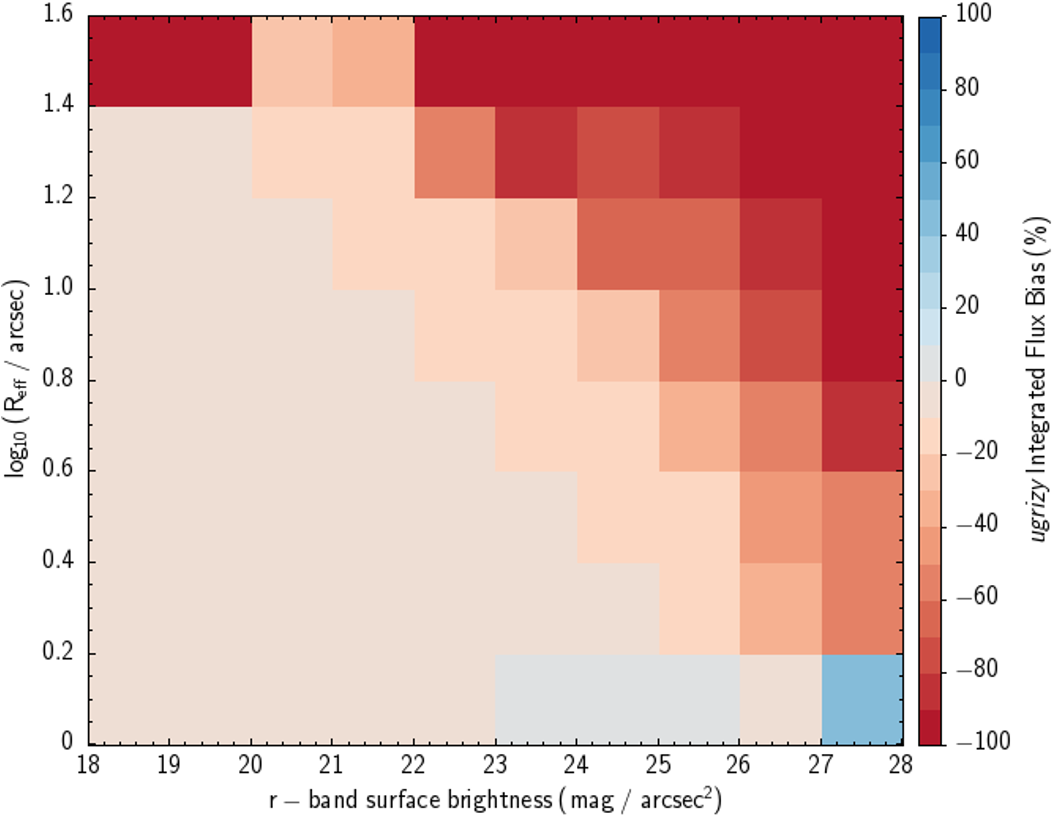
\includegraphics[width=\textwidth]{figures/flux_bias_sb_vs_reff}
  \caption{Median $ugrizy$ integrated flux bias (\%) as a function of
    $r$-band surface brightness ($x$-axis) and $\log(\Reff/\mathrm{arcsec})$
    ($y$-axis). Red shading: flux underestimation (negative bias). Blue
    shading: flux overestimation. At $\log \Reff > 1.2$ ($\Reff \gtrsim
    15$~arcsec), the flux is systematically underestimated by $40$--$100\%$.
    At $\log \Reff < 0.2$ ($\Reff \lesssim 1.5$~arcsec) and $\mur > 26$,
    the flux is overestimated.}
  \label{fig:2d_bias}
\end{figure}

This figure reveals the full structure of the bias. At the top of the diagram
($\log \Reff > 1.2$, i.e.\ $\Reff \gtrsim 15$~arcsec), the flux is
underestimated by $40$--$100\%$ at all surface brightnesses. This is the
regime in which shredding by spurious detections dominates. At the bottom
($\log \Reff < 0.4$, i.e.\ $\Reff \lesssim 2.5$~arcsec), the bias
transitions to an overestimate for $\mur > 25$. The transition from
underestimation to overestimation occurs at $\Reff \sim 3$--$5$~arcsec. We
note that this transition radius is of order several times the LSST PSF FWHM
(${\sim}0.7$~arcsec), suggesting that the distinction between `resolved' and
`unresolved' in the context of \scarlet's morphological fitting governs the
direction of the bias.

An important caveat applies to the interpretation of the flux underestimate
for extended sources. Our source-matching procedure assigns the injected source
the single detection closest to the injection position. If the source has been
shredded into multiple child detections, only one child is matched, and the
remainder of the flux resides in spurious children within the same Footprint.
The measured `flux loss' therefore reflects the flux assigned to the matched
child alone, and may overestimate the true flux deficit if the total flux
across all children is closer to conserved. We return to this point in
Section~\ref{sec:nextsteps} (flux reassembly).

\subsection{Detection and Stellar Mass Bias vs.\ Stellar Mass}
\label{sec:mass_bias}

Up to this point all performance metrics have been measured as a function of
surface brightness and radius. It is also of use to examine performance as a
function of physical galaxy parameters, such as stellar mass. In much the same
way as shown with Figures~\ref{fig:kde_marginals} and~\ref{fig:cosmos_properties},
we bin by stellar mass and draw 100 realistic sets of galaxy properties at
each stellar mass (bins of 0.5~dex), drawing randomly from the distributions
found for the COSMOS-UltraVISTA dataset.

Figure~\ref{fig:mass_bias} shows the detection fraction and stellar mass
bias as a function of input stellar mass.

\begin{figure}
  \centering
  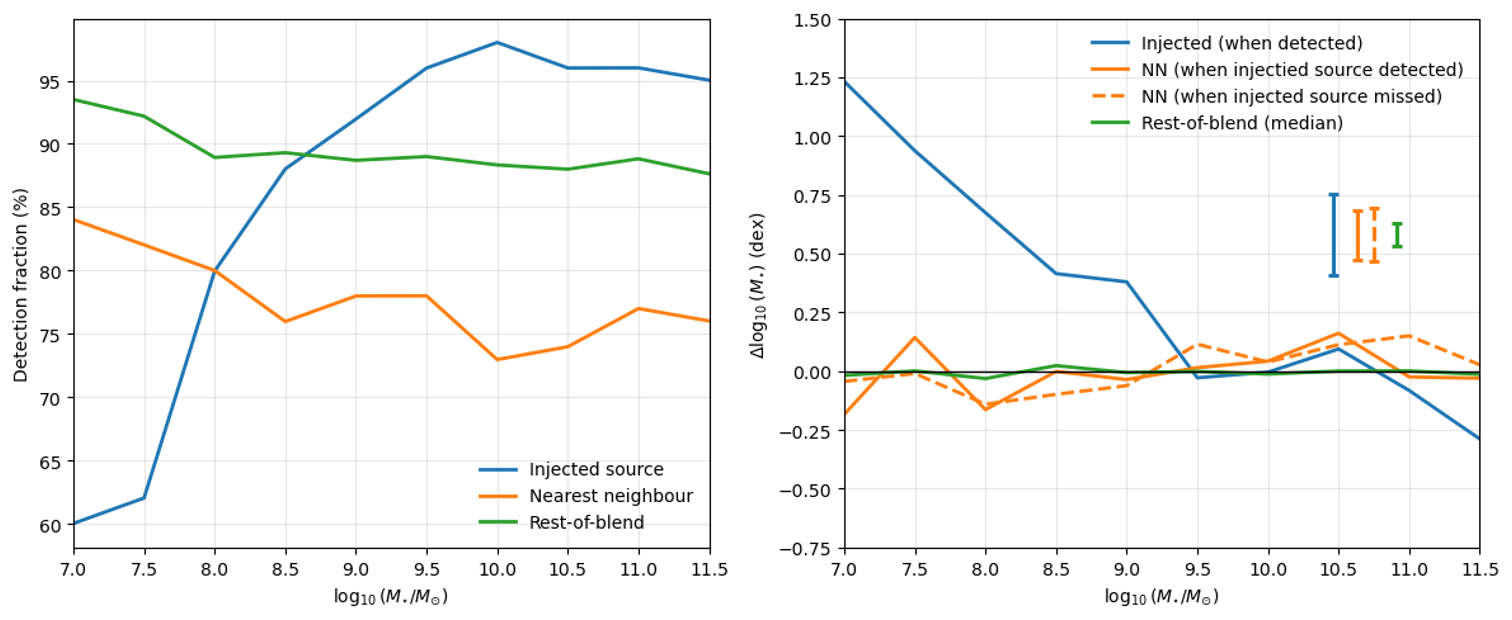
\includegraphics[width=\textwidth]{figures/detection_stellar_mass_bias}
  \caption{Left: detection fraction vs.\ input stellar mass
    $\log(\Mstar/\Msun)$. Blue: injected source. Orange: nearest neighbour.
    Green: rest of blend. Right: stellar mass bias $\Delta \log M_*$ (dex)
    for detected sources. Error bars show the interquartile range at selected
    mass bins.}
  \label{fig:mass_bias}
\end{figure}

The injected-source detection fraction dips to ${\sim}75\%$ at
$\log(\Mstar/\Msun) \sim 8.0$, driven by the low surface brightnesses typical
of galaxies at this mass scale, and recovers to ${>}95\%$ at
$\log(\Mstar/\Msun) > 9.5$. The stellar mass bias for detected injected sources
is generally ${<}0.2$~dex. However, the nearest-neighbour mass is biased by up
to $+0.25$~dex when the injection is detected (solid orange), indicating excess
flux attribution from the wings of the injected source model.

\subsection{Impact on the Galaxy Stellar Mass Function}
\label{sec:gsmf}

To illustrate the downstream scientific impact, we apply the measured
detection fractions and mass biases from Experiment~1 to the
COSMOS-UltraVISTA catalogue ($z < 0.4$) and compare the predicted GSMF with
the observed LSST GSMF. Figure~\ref{fig:gsmf} shows three curves: the
COSMOS-UltraVISTA GSMF (blue), the LSST catalogue GSMF (orange), and the
COSMOS-UltraVISTA GSMF after applying our measured detection and deblender
biases (green).

\begin{figure}
  \centering
  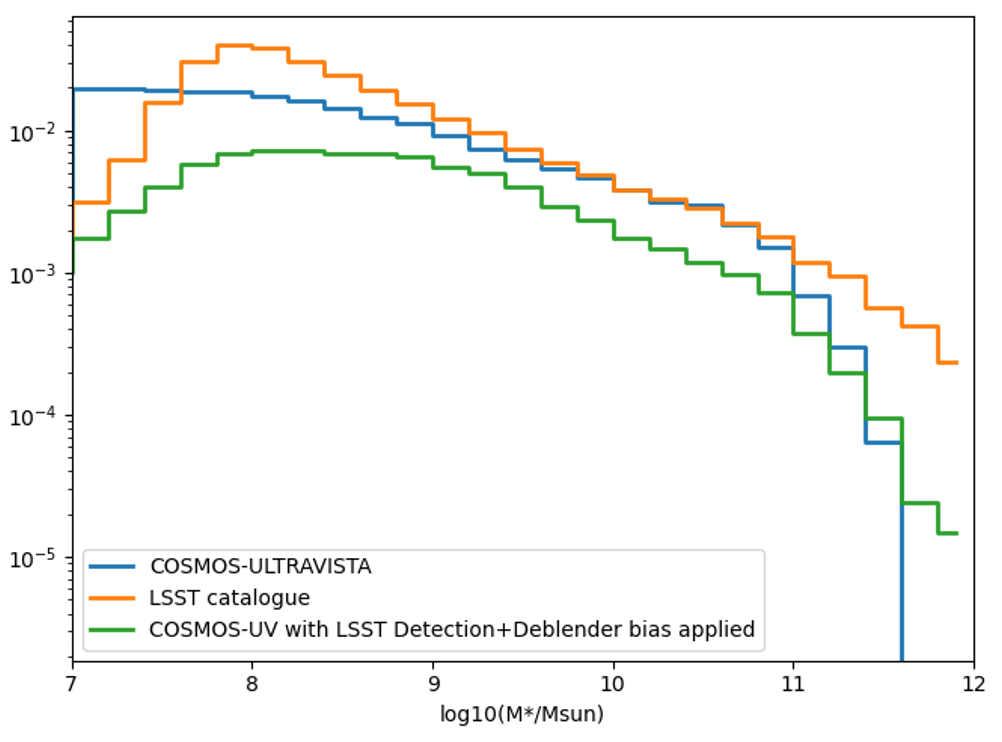
\includegraphics[width=0.85\textwidth]{figures/galaxy_stellar_mass_function}
  \caption{The galaxy stellar mass function (normalised number density per
    dex). Blue: COSMOS-UltraVISTA ($z < 0.4$). Orange: LSST object catalogue
    (matched area). Green: COSMOS-UltraVISTA with the measured LSST detection
    and deblender bias applied. The LSST GSMF shows a ${\sim}0.5$~dex excess
    at $\log(\Mstar/\Msun) \sim 8$ relative to COSMOS. The bias-corrected
    COSMOS GSMF shows a deficit reaching ${\sim}1$~dex at
    $\log(\Mstar/\Msun) < 8$.}
  \label{fig:gsmf}
\end{figure}

The LSST GSMF (orange) shows a systematic excess at $\log(\Mstar/\Msun) \sim
7.5$--$8.5$, peaking at approximately $0.5$~dex above the COSMOS reference.
This excess is consistent with the flux overestimate for faint, compact sources
(Section~\ref{sec:2d_bias}). The bias-corrected COSMOS GSMF (green) shows a
deficit at all masses below $\log(\Mstar/\Msun) \sim 10$, reaching ${\sim}1$~dex
at the lowest masses. Together, these effects produce a GSMF that is
unreliable below $\log(\Mstar/\Msun) \sim 9$.

We note two caveats in this comparison. First, the COSMOS stellar masses are
SED-fit catalogue products from \citet{Weaver2022}, whereas the LSST masses
are derived from the pipeline-measured photometry using the \citet{Bryant2015}
prescription; differences in the stellar mass estimators may contribute to the
offset at the high-mass end. Second, cosmic variance between the COSMOS and
LSST footprints, and differences in area and depth, mean that the
normalisation of the two GSMFs is not expected to agree precisely. The
qualitative shape of the discrepancy, rather than its absolute normalisation,
is the primary diagnostic.


% =============================================================================
\section{ICL-like Extended Source Injection Experiment}
\label{sec:icl_experiment}
% =============================================================================

The results of Sections~\ref{sec:exp2} and~\ref{sec:2d_bias} demonstrate
that extendedness is the primary driver of flux underestimation and
source fragmentation in the current pipeline. To probe this regime more
directly, we designed a dedicated injection experiment using
intracluster-light-like (ICL-like) synthetic sources whose surface
brightness profiles extend to considerably larger angular scales than the
NewHorizon dwarf galaxies employed in the preceding sections.

\subsection{ICL Source Model}
\label{sec:icl_model}

We model the injected ICL-like sources using the core-S\'{e}rsic profile
\citep{Graham2003}, which provides a smooth connection between an outer
S\'{e}rsic component and an inner power-law component. The core-S\'{e}rsic
profile can be expressed as
\begin{equation}
  I(R) = I' \left[1 + \left(\frac{R_{b,\mathrm{cS}}}{R}\right)^{\!\alpha}\right]^{\!\gamma/\alpha}
         \exp\!\left[-b_n\left(\frac{R^{\alpha} + R_b^{\alpha}}
                                    {R_e^{\alpha}}\right)^{\!1/(n\alpha)}\right],
  \label{eq:core_sersic}
\end{equation}
where $R_e$ is the effective radius, $R_{b,\mathrm{cS}}$ the break
(core) radius, $n$ the S\'{e}rsic index, $\alpha$ the sharpness of the
transition between the inner power law and the outer S\'{e}rsic profile,
$\gamma$ the logarithmic slope of the inner power law, and $b_n$ is
defined such that $R_e$ encloses half the total model luminosity. The
normalisation $I'$ is set by the target peak surface brightness $\mu_b$.
We adopt parameters representative of the brightest cluster galaxy
A2261-BCG as determined by \citet{BonfiniGraham2016}: $n = 3.9$,
$\alpha = 3.6$, $\gamma = 0.02$, and $R_b / R_e = 0.12$. We assume an
axis ratio $q = 0.7$ and a random position angle, and render the 2D
profile in the LSST $r$ band. Multi-band fluxes are generated by
applying a uniform old-stellar-population colour gradient consistent
with typical ICL observations.

\subsection{Experimental Design}
\label{sec:icl_design}

We vary two parameters: the effective radius $R_e \in [5, 60]$~arcsec
and the peak surface brightness $\mu_b \in [20, 28]$~$\mathrm{mag\,arcsec^{-2}}$.
Injections are performed into a single patch (patch~83, tract~9812) to
hold the background and crowding conditions fixed, with one injection per
$(R_e, \mu_b)$ bin. As in the preceding experiments, we process the
modified single-exposure images through the full LSST pipeline and
compare the resulting catalogues against the pre-injection baseline. For
each bin we compute: (i)~the number of real sources lost after
injection; (ii)~the number of new (spurious) sources created by the
pipeline; (iii)~the total flux attributed to new detections relative
to the injected flux; (iv)~the fraction of this flux assigned to the
primary (nearest-to-core) detection; (v)~the aggregated flux bias over
the entire scene; and (vi)~the median $r$-band flux change of surviving
pre-injection neighbours.

\subsection{Detection Disruption}
\label{sec:icl_detection}

Figure~\ref{fig:icl_det_spurious} presents the impact of the presence of an ICL-like source on detection: through both the loss of real
detections and the creation of spurious ones. 

The left panel shows the
number of new detections (not detected within 5 pixels of their centroid position before injection)
introduced by the injecton of a single extended source. For the brightest and most extended injected sources ($\mu_b \lesssim 22$, $R_e \gtrsim 30$~arcsec),
of order $10^3$ spurious sources are created. It appear that despite the smooth sersic nature of injections, 
the impact of real sources in both the signal and variance plane causes the peak finding algorithm to produce spurious detections.

The right panel shows the
corresponding number of real sources that were detected in the pre-injection catalogue
but are absent (within a 5 pixel tolerance) from the post-injection catalogue within the footprint of
the injected profile, with of order $10^3$ real
sources lost from the catalogue due to the presence of the diffuse flux.

\begin{figure}
  \centering
  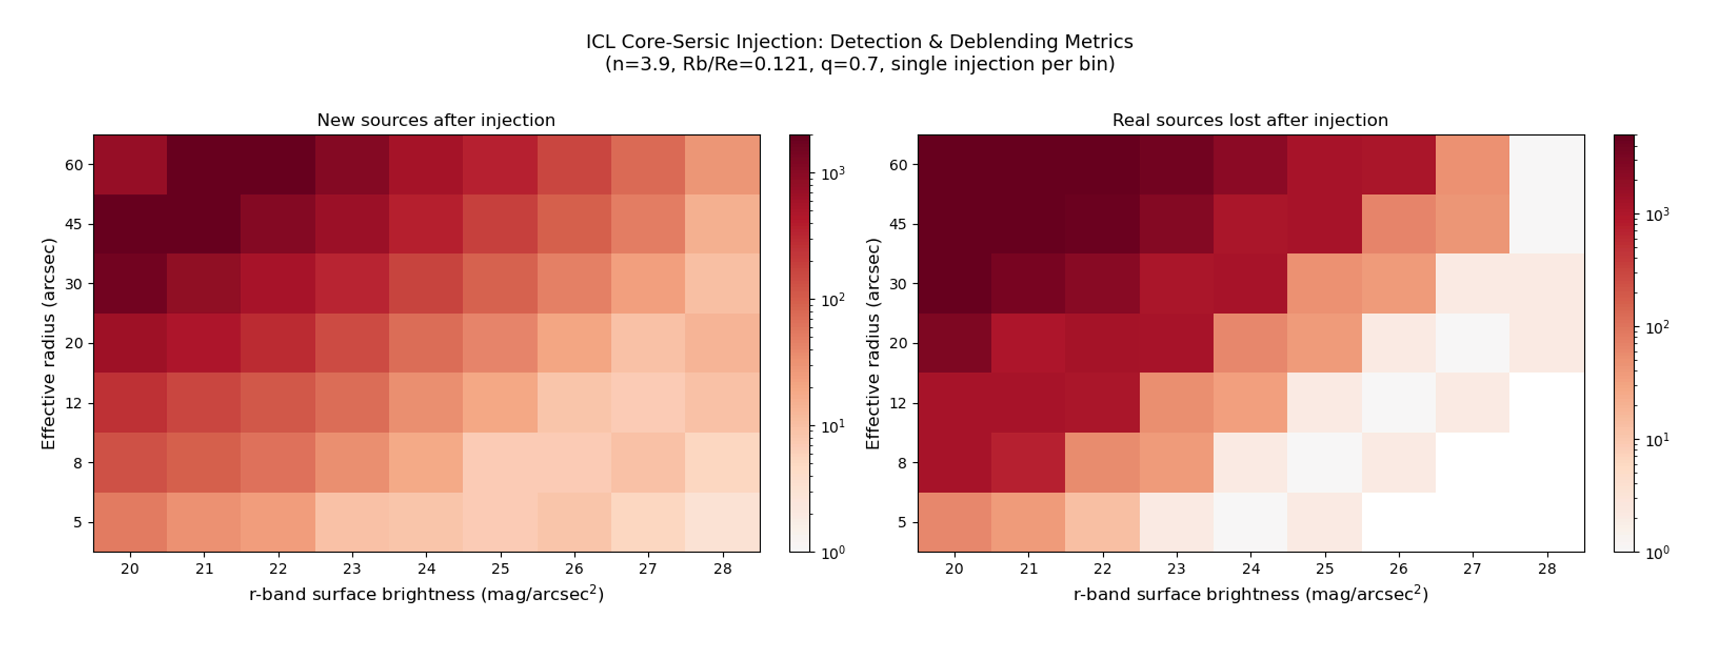
\includegraphics[width=\textwidth]{figures/icl_detection_lost_spurious}
  \caption{Detection disruption from ICL-like core-S\'{e}rsic injections as a
    function of $r$-band peak surface brightness ($x$-axis) and effective
    radius ($y$-axis). \textit{Left}: number of new (spurious) sources
    created by the detection pipeline within the injected source's footprint. \textit{Right}: number of real sources lost from the
    catalogue after injection.
    In both panels, the most extended and brightest injections ($R_e \gtrsim 30$~arcsec,
    $\mu_b \lesssim 22$) produce of order $10^3$ lost and $10^3$ spurious
    detections.}
  \label{fig:icl_det_spurious}
\end{figure}

\subsection{Flux Bias}
\label{sec:icl_flux}

Figure~\ref{fig:icl_flux_bias} presents four complementary flux
diagnostics. The upper-left panel shows the total flux attributed by the
pipeline to new detections (not found within a 5 pixel tolerence before injection) as a percentage of the true injected flux.
For the brightest, most extended injections ($\mu_b \lesssim 22$, $R_e \gtrsim
30$~arcsec), the summed flux of the spurious sources exceeds the
injected flux by more than an order of magnitude. This precludes a straightforward post-hoc correction
in which one simply sums the flux of shredded components to reconstruct extended sources.

The upper-right panel shows the flux bias of the primary new detection
(defined as the detection nearest to the profile centre). Over a wide range of surface brightnesses,
this source captures only a small fraction of the total
injected flux, reemphasising the fact that the ICL emission is distributed
across many child sources. 

The lower-left panel presents the aggregated scene flux bias: the
difference between the total flux of all detected sources within the
injection footprint after injection and the corresponding total before
injection in the same footprint, minus the known injected flux, normalised by the injected
flux. If the pipeline were to perfectly conserve flux, this quantity
would equal zero. Instead, bright and extended ICL-like injections
produce scene-level flux errors of order $50$--$100\%$ in both
directions (overestimation and underestimation), while more compact and
fainter injections show a persistent underestimate of the total scene
flux, albeit of smaller magnitude.

Finally, the lower-right panel shows the median $r$-band flux bias of
surviving pre-injection neighbours within the post-injection blend mask: real sources that were detected
both before and after injection (within a 5 pixel tolerance). The median
neighbour flux bias is found to be positive across the entire $(R_e, \mu_b)$ gridspace.
Sources embedded in diffuse ICL-like emission systematically gain flux.
The effect is present for all but the faintest, most compact injections.
This result demonstrates that the deblender systematically misattributes a portion of the diffuse ICL
emission to pre-existing sources rather than to a single extended
component.

\begin{figure}
  \centering
  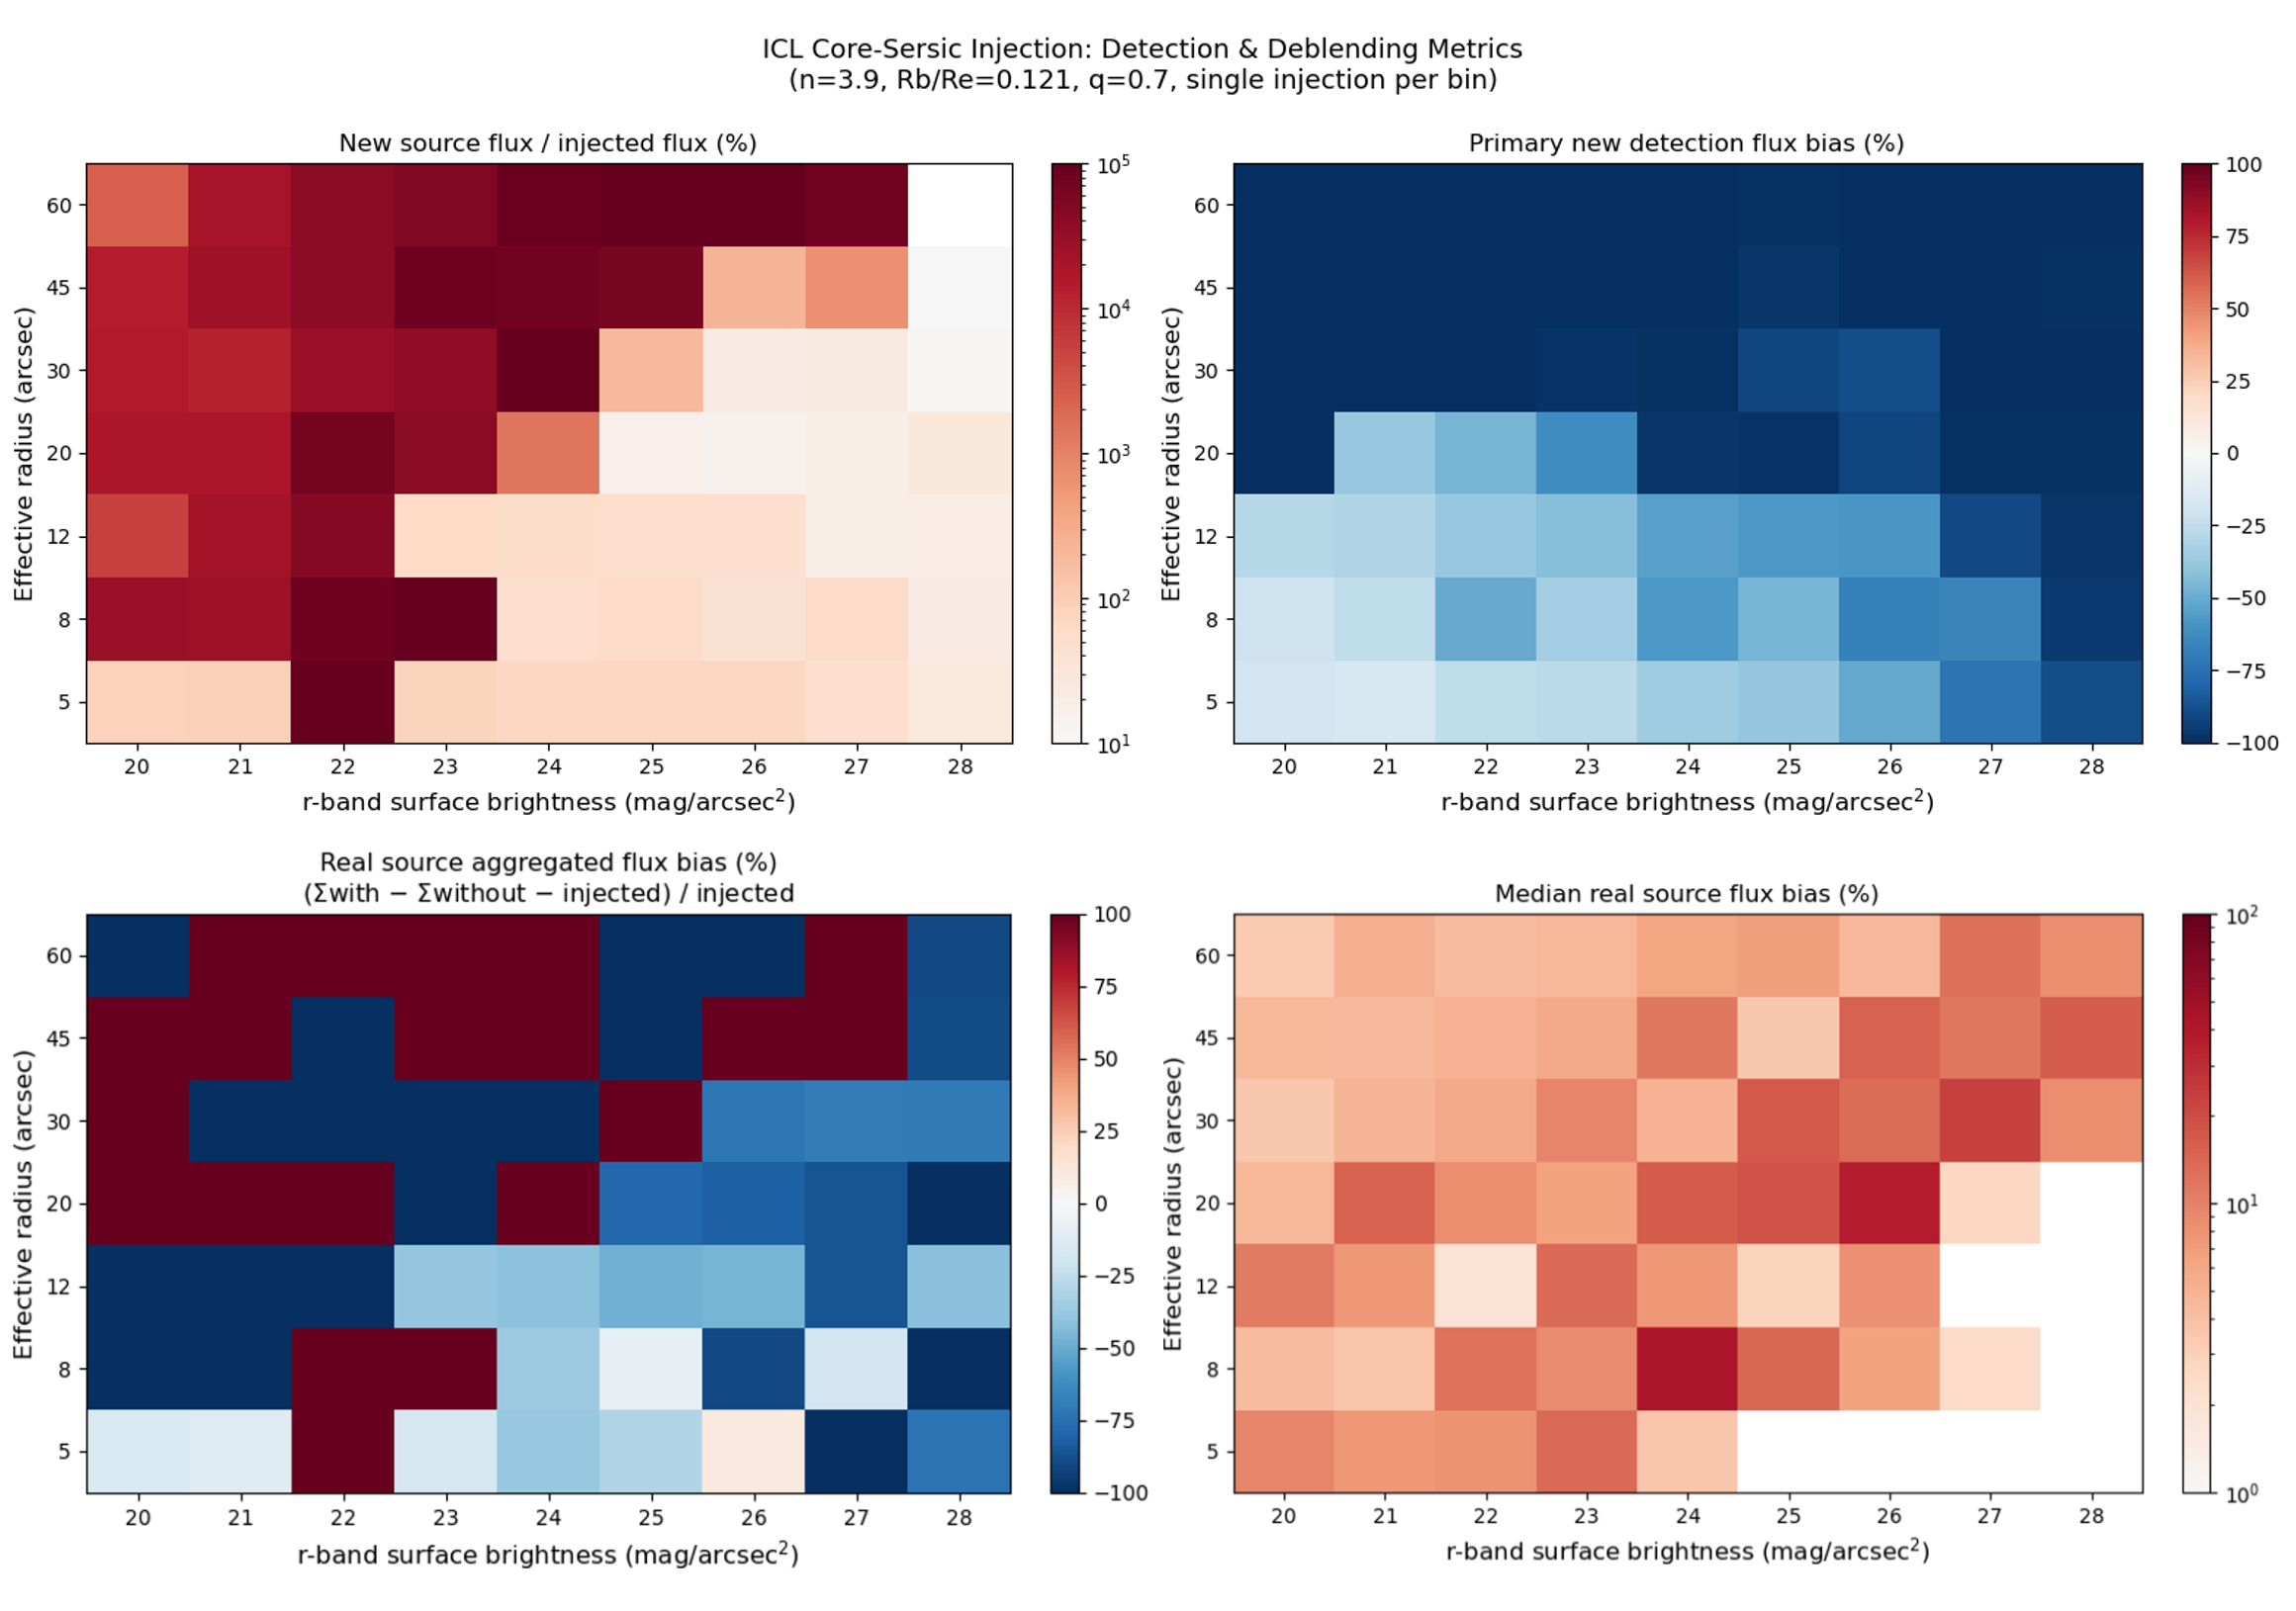
\includegraphics[width=\textwidth]{figures/icl_flux_bias_panels}
  \caption{Flux bias diagnostics for ICL-like core-S\'{e}rsic injections.
    \textit{Upper left}: total flux of new (spurious) detections as a percentage
    of the injected flux. Values exceeding $100\%$ indicate that the pipeline
    attributes more flux to new sources than was injected.
    \textit{Upper right}: $r$-band flux bias of the primary new detection
    (nearest to the core).
    \textit{Lower left}: aggregated scene flux bias
    ($[\Sigma F_{\rm with} - \Sigma F_{\rm without} - F_{\rm injected}] /
      F_{\rm injected}$), measuring net flux non-conservation.
    \textit{Lower right}: median $r$-band flux change of surviving
    pre-injection neighbours. Positive values (red) indicate flux overestimation;
    negative values (blue) indicate underestimation.}
  \label{fig:icl_flux_bias}
\end{figure}


% =============================================================================
\section{Implications for LSST Science Cases}
\label{sec:implications}
% =============================================================================

The biases quantified above have direct consequences for several key LSST
science drivers. We briefly discuss the most affected areas.

\subsection{Dwarf Galaxy Demographics and the Faint-End GSMF}
\label{sec:implications_dwarfs}

The faint-end slope of the GSMF is a critical observable for constraining
galaxy formation models \citep[e.g.][]{Benson2003,Baldry2012} and the nature
of dark matter \citep[e.g.][]{BullockBoylanKolchin2017}. Our results show
that the current pipeline introduces a detection completeness drop to
${<}50\%$ at $\mur = 25$~$\mathrm{mag\,arcsec^{-2}}$, precisely the regime
populated by many dwarf galaxies and ultra-diffuse galaxies
\citep{vanDokkum2015,Martin2019}. The surviving detected dwarfs are subject
to flux biases of up to a factor of 10. Any measurement of the faint-end
slope from LSST catalogues will therefore require careful completeness and
bias corrections. As shown in Figure~\ref{fig:mass_bias}, we predict that
the galaxy stellar mass function as derived from scarlet-produced object catalogues
would exhibit a substantial overestimate in number density at $10^8$ M$_{\odot}$
and a yet more severe underestimate in number density at $10^7$ M$_{\odot}$ and below.
Such biased results would lead to inaccurate conclusions for the nature of the cosmology.
Work must be undertaken to: (i) optimise the peak finding algorithm to better catch the faintest compact sources, and
(ii) attribute flux to blended sources more reliably in the LSB regime.

\subsection{Intracluster Light}
\label{sec:implications_icl}

Measurements of the ICL fraction in galaxy clusters
\citep[e.g.][]{Montes2019,Kluge2021} depend sensitively on the ability of
the deblender to separate diffuse ICL from the envelopes of bright cluster
galaxies. The ${\sim}40$--$100\%$ flux underestimate we find for extended
sources ($\Reff > 15$~arcsec; Figure~\ref{fig:2d_bias}) indicates that a
substantial fraction of extended source flux is being lost to shredding.
The dedicated ICL-like injection experiment
(Section~\ref{sec:icl_experiment}) confirms this picture:
injections with $R_e \gtrsim 30$~arcsec and $\mu_b \lesssim 22$ produce of
order $10^3$ spurious detections and cause the loss of a comparable number
of real sources in their vicinity, while the total flux attributed
to spurious objects exceeds the injected flux by more than an order of magnitude.
These results indicate that the current pipeline, which was designed and optimised
for the galaxy-scale regime, does not perform reliably upon ICL-scale diffuse
emission in its present form. Figure~\ref{fig:icl_flux_bias} indicates that
a simple post procesing step to recombine shredded components in extended sources is unlikely to be sufficient.
As such, any measurement of the ICL fraction from
LSST catalogues will therefore require at least one of the following:
(i) adjustments to the current peak-detection implementation,
(ii) relaxation of \scarlet's monotonicity constraints,
(iii) a dedicated spurious-detection suppression step prior to deblending, or
(iv) an ICL-extraction step upstream of the standard detection pipeline.

\subsection{Weak Gravitational Lensing}
\label{sec:implications_wl}

Weak-lensing shear estimation \citep[e.g.][]{SheldonHuff2017,Mandelbaum2018}
relies on accurate galaxy shape measurements, which in turn require unbiased flux
and morphology models. The flux redistribution and morphological distortion we
observe, both for injected sources and their neighbours, risk contaminating
the effective PSF model used for shape measurement. Given the stringent LSST DESC
limit on multiplicative shear bias ($|m| < 0.003$; \citealt{LSST_DESC2018}), it
is important to determine whether deblending systematics contribute at this level.

\subsection{Strong Lensing}
\label{sec:implications_sl}

Strong gravitational lensing studies require accurate photometry and
morphology of lensed arcs, Einstein rings, and multiply-imaged sources
\citep[e.g.][]{Suyu2017}. These features are typically extended, low surface
brightness, and embedded in complex blends with the lens galaxy. The shredding
and left-behind flux failure modes are expected to be particularly severe for
these configurations.

\subsection{Transient Science and Host Galaxy Association}
\label{sec:implications_transients}

The association of transient events (supernovae, kilonovae, tidal disruption
events) with their host galaxies depends on accurate source catalogues in the
vicinity of the transient \citep[e.g.][]{Gupta2016,Foley2013,Sako2018}. The
detection loss of neighbours in the vicinity of bright sources and the
shredding of extended hosts could lead to incorrect host-galaxy
identification, propagating into biased host-galaxy properties and, for Type
Ia supernovae, into biased cosmological distance estimates.

\subsection{Photometric Redshifts}
\label{sec:implications_photoz}

Photometric redshift estimation \citep[e.g.][]{Benitez2000} requires accurate
multi-band photometry. The colour-dependent flux biases introduced by the
deblender, particularly the monotonicity-driven underestimate of flux in
non-monotonic features with distinct colours from the source centre, will
distort the SED used for photo-$z$ estimation.


% =============================================================================
\section{Summary}
\label{sec:summary}
% =============================================================================

We have presented a quantitative assessment of the LSST detection and
deblending pipeline (\task{SourceDetectionTask} + \task{ScarletDeblendTask})
using controlled injection experiments on real LSSTCam deep coadds. Our
principal findings are as follows:

\begin{enumerate}
  \item \textbf{Detection completeness.} The detection fraction of injected
    sources drops from ${\sim}95\%$ at $\mur = 20$~$\mathrm{mag\,arcsec^{-2}}$
    to ${\sim}50\%$ at $\mur = 25$ and ${\sim}10\%$ at $\mur = 27$.

  \item \textbf{Flux overestimate for faint, compact sources.} In the
    realistic (COSMOS-drawn) experiment, the recovered $r$-band flux is
    overestimated by ${\sim}100\%$ (a factor of ${\sim}2$) at $\mur = 27$,
    and by approximately an order of magnitude at $\mur = 30$
    $\mathrm{mag\,arcsec^{-2}}$ (bias $+900\%$, equivalent to ${\sim}2.5$~mag).

  \item \textbf{Flux underestimate for extended sources.} In the controlled
    experiment (fixed $\Reff = 5$~arcsec), the recovered flux is increasingly
    underestimated at fainter surface brightnesses, reaching ${\sim}50$--$60\%$
    underestimate at $\mur = 26$. In the 2D analysis, sources with $\Reff
    \gtrsim 15$~arcsec show flux underestimates of $40$--$100\%$ irrespective
    of surface brightness (though see Section~\ref{sec:2d_bias} caveat
    regarding flux redistribution among shredded children).

  \item \textbf{Neighbour impact.} The injection of a bright source ($\mur =
    18$) causes ${\sim}60\%$ of nearest-neighbour detections to be lost. Even
    faint injections ($\mur = 30$) cause ${\sim}20\%$ neighbour loss.
    Nearest-neighbour stellar masses are biased by up to $+0.25$~dex.

  \item \textbf{Extendedness governs bias direction.} The 2D $\mur$ vs.\
    \Reff analysis (Figure~\ref{fig:2d_bias}) demonstrates that the transition
    from underestimation to overestimation occurs at $\Reff \sim 3$--$5$~arcsec.

  \item \textbf{GSMF distortion.} The combined effect of detection
    incompleteness and photometric bias produces a GSMF that is unreliable
    below $\log(\Mstar/\Msun) \sim 9$, with a ${\sim}0.5$~dex excess at
    $\log(\Mstar/\Msun) \sim 8$ and a ${\sim}1$~dex deficit at
    $\log(\Mstar/\Msun) < 8$.

  \item \textbf{Current limitations for ICL-like extended emission.} A
    dedicated experiment injecting core-S\'{e}rsic profiles with effective
    radii up to 60~arcsec confirms that extendedness is the primary
    challenge for the current detection and deblending algorithms. For the
    most extended and
    brightest ICL-like injections ($R_e \gtrsim 30$~arcsec,
    $\mu_b \lesssim 22$~$\mathrm{mag\,arcsec^{-2}}$), the pipeline
    creates of order $10^3$ spurious detections and simultaneously removes
    a comparable number of real sources from the catalogue. The total flux
    assigned to spurious detections exceeds the injected flux by more than
    an order of magnitude, and the primary detection nearest the profile
    core captures only a small fraction of the injected light. Surviving
    neighbours embedded in the diffuse emission systematically gain flux,
    with a positive median flux bias across essentially the entire
    parameter space.
\end{enumerate}


% =============================================================================
\section{Next Steps}
\label{sec:nextsteps}
% =============================================================================

The results presented above motivate several avenues of further work, which
we outline below.

\paragraph{Morphological priors for \scarlet.}
The current \scarlet implementation uses entirely non-parametric morphologies
with no prior on the shape of $\mathbf{S}_k$ beyond monotonicity and
(optionally) symmetry. Introducing a data-driven morphological prior on the range of
reasonable morphologies for disturbed, interacting and isolated galaxies
could regularise the deblender towards physically plausible galaxy shapes. 
Recent work on score-matching neural networks for galaxy morphology priors \citep{Sampson2024} offers a promising
avenue for integrating learned priors into the \scarlet framework.

\paragraph{Improved detection of extended sources.}
The shredding failure mode arises from the \task{DetectCoaddSourcesTask}
placing spurious peaks within extended galaxies. Developing scale-dependent
detection thresholds, or a spatially aware detection scheme that better considers the flux
in adjacent pixels could reduce the rate of spurious detections.
An iterative feedback loop between the deblender and the detector, in which \scarlet flags peaks with
implausible models for rejection, would also mitigate this failure mode.

\paragraph{Conditional relaxation of the monotonicity constraint.}
The monotonicity constraint is found to often be responsible for the left-behind flux failure
mode in sources with structure such as star-forming regions and spiral arms. A conditional
approach, in which the constraint is relaxed for sources above a configurable
signal-to-noise threshold or spatial extent, could improve flux recovery for
late-type galaxies while retaining the regularisation benefits for faint or
poorly resolved sources.

\paragraph{Flux reassembly for shredded sources.}
Our ICL injection results (Section~\ref{sec:icl_experiment}) show that naive
reassembly of child-source fluxes within the injection footprint does not recover
the true injected flux, when examined over a wide range of surface brightness and
source extendedness. Even if \scarlet\ sources could be reliably flagged for
recombination, our findings indicate that a simple flux summation is unlikely to
be sufficient; any viable correction for shredded sources will therefore require a
more sophisticated approach which would warrant further investigation,
and the first priority would be to avoid the shredding of galaxies to occur prior to deblending.

\paragraph{Downstream science impact studies.}
Dedicated injection experiments should be performed within the shape
measurement pipeline (for weak lensing shear bias; cf.\ \citealt{LSST_DESC2018}),
the photometric redshift pipeline, and the transient host-galaxy association
pipeline. We encourage members of the relevant LSST science collaborations
(DESC, SMWLV, TVS, LSB) to engage with these results.

\smallskip
In summary, the current LSST detection and deblending pipeline introduces
systematic biases that are significant across a wide range of galaxy
properties, not only in the LSB regime. We stress the importance of
quantifying and addressing these biases as early as possible,
in order to maximise the long-term scientific output of Rubin.

\smallskip
\noindent\textit{Note on continuity:} Due to funding constraints this work
will likely need to be continued by a team outside of WP:UKD-UKD-S6 from
March 2026 onwards.


\appendix

\section{Acknowledgements}

This material is based upon work supported in part by the National Science
Foundation through Cooperative Agreements AST-1258333 and AST-2241526 and
Cooperative Support Agreements AST-1202910 and AST-2211468 managed by the
Association of Universities for Research in Astronomy (AURA), and the
Department of Energy under Contract No.\ DE-AC02-76SF00515 with the SLAC
National Accelerator Laboratory managed by Stanford University.
Additional Rubin Observatory funding comes from private donations, grants to
universities, and in-kind support from LSST-DA Institutional Members.
T.M.S.\ acknowledges support from the University of Hertfordshire and
participation as an external member of Rubin Data Management
(WP:UKD-UKD-S6).
The injection experiments were performed in collaboration with F.\ Moolekamp,
L.\ Kelvin, A.\ Watkins, S.\ Kaviraj, and C.\ Collins.

% Include all the relevant bib files.
% https://lsst-texmf.lsst.io/lsstdoc.html#bibliographies
\section{References} \label{sec:bib}
\renewcommand{\refname}{} % Suppress default Bibliography section
\bibliography{local,lsst,lsst-dm,refs_ads,refs,books}

% Make sure lsst-texmf/bin/generateAcronyms.py is in your path
\section{Acronyms} \label{sec:acronyms}
\input{acronyms.tex}
% If you want glossary uncomment below -- comment out the two lines above
%\printglossaries


\end{document}
